\documentclass[11pt,a4paper]{article}
\usepackage[utf8]{inputenc}  % .tex chars encoding
\usepackage[T1]{fontenc}     % .pdf chars encoding
\usepackage[italian]{babel}  % translations
\usepackage{amsmath}         % math symbols
\usepackage{amsfonts}        % extended math symbols
\usepackage{amssymb}         % other math symbols
\usepackage{hyperref}        % hyperref
\usepackage{graphicx}        % images
\usepackage{float}           % float options

% Macros
% ======
\newcommand*{\wix}{Wix}
\newcommand*{\wixcom}{wix.com}
\newcommand*{\wixcome}{\emph{\wixcom{}}}

% Configs
% =======

% Path relative to the main .tex file 
\graphicspath{ {./img/} }

\author{Luca Parolari}
\title{Web Information Management\\ \large Analisi di usabilità del sito web \wixcom{}}

% Document
% ========

\begin{document}

\maketitle

\clearpage
\tableofcontents

\clearpage

\section{Introduzione}
\label{sec:intro}

Questo documento si prefigge lo scopo di fornire un'analisi di
usabilità del sito web \href{https://wix.com}{\wixcom{}}. Il sito web è
stato analizzato nel periodo di gennaio 2021.

\begin{figure}[h]
  \centering
  
\includegraphics[width=0.25\textwidth]{wix-logo}
  \caption{Logo di \wix{}}
  \label{fix:wix-logo}
\end{figure}

\wix{} promuove il suo prodotto principale: un site builder fruibile da
tutti gli utenti sia con che senza conoscenza informatica. I suoi
obiettivi principali sono rendere semplice, immediata, user-friendly e
gratuita la manutenzione del proprio sito web online offrendo
strumenti integrati nel site builder per costruire e modificare blog,
e-commerce e siti vetrina.

\section{Analisi preliminare}
\label{sec:preliminary-analysis}

\subsection{Contesto}
\label{subsec:context}

\wix{}, in linea generale, è un site builder. Un site builder è uno
strumento software che tipicamente permette la costruzione di siti web
senza (o quasi) scrivere del codice
manualmente.\footnote{\url{https://en.wikipedia.org/wiki/Website_builder}}.
I
site builder si distinguono in due macro categorie: \emph{online} site
builder, dove lo strumento è fornito in cloud ed è gestito
privatamente dal provider che offre il servizio e lo spazio dove
hostare il proprio sito web e \emph{offline} site builder dove invece
lo strumento può essere eseguito sul computer e genera le pagine del
sito che possono poi essere distribuite su un qualunque web hosting.

\wix{} rientra chiaramente nella prima categoria: l'output generato
dal sitebuilder di \wix{} non può essere esportato su altri
provider. Questo rappresenta infatti il core-business di \wix{}: un
servizio di hosting con un grandissimo valore aggiungo, ovvero il site
builder. 

\subsection{Nome del sito}
\label{subsec:site-name}

Il nome \wix{} è ben fatto e segue delle regole ben precise. Esso infatti è

\begin{itemize}
  \item unico;
  \item corto a tal punto che è composto dal minimo numero di lettere
    per creare un nome orecchiabile;
  \item facile da memorizzare e da scrivere, anche se presenta lettere
    come la \emph{w} e la \emph{x} provenienti dall'afabeto
    internazionale e non originariamente presenti nell'afabeto
    italiano. Quest'ultime però sono ormai state sdoganate e tutti ne
    conoscono l'esistenza;
  \item seguito dal dominio ``.com'', molto famoso e facile da
    indovinare anche se non memorizzato;
\end{itemize}

Inoltre, il nome \wix{} risulta correttamente registrato (controllo eseguito su \href{https://www3.wipo.int/branddb/en/}{WIPO
  Global Brand Database}).


\section{Homepage}
\label{sec:homepage-analysis}

Nella sezione \ref{subsec:homepage-description} viene descritta la
homepage screen per screen dato lo sviluppo verticale della pagina,
mentre in \ref{subsec:homepage-the-six-ws} viene argomentata le
gestione delle informazioni per quanto riguarda i sei assi informativi
della pagina web.

\subsection{Descrizione generale}
\label{subsec:homepage-description}

Dall'URL \url{https://wix.com} si accede alla homapage del sito
\wix{}. La figura \ref{fig:homepage-01} mostra la schermata più
importante del sito web, ovvero quella visibile senza alcuno scroll e
quindi accessibile da tutti gli utenti.

L'entry point di questa pagina è il logo di \wix{} che occupa, con del
testo, esattamente la posizione in alto a sinistra della pagina. Il
menu poi prosegue con alcune voci per navigare il sito ed un pulsante
\textit{Accedi}, che probabilmente viene utilizzato dagli utenti
ricorrenti per accedere al proprio account. L'unica parte veramente
informativa della pagina è il titolo nel mezzo dell'immagine: ``Crea
il tuo sito web professionale'', che lascia intuire l'obiettivo del
sito ma non lo esplicita completamente. Dal punto di vista informativo
questa pagina è molto povera e sicuramente non riesce a soddisfare le
richieste dell'utente, il quale vorrebbe per lo meno capire in che
sito web è capitato.

Il click sul pulsante \textit{Inizia} non porta ad ulteriori
informazioni, bensì ad una pagina di accesso/registrazione: siamo di
fronte al problema della registrazione prematura, in quanto in questa
fase, un utente nuovo, non ha ancora capito lo scopo del sito.

\begin{figure}[H]
  \centering
  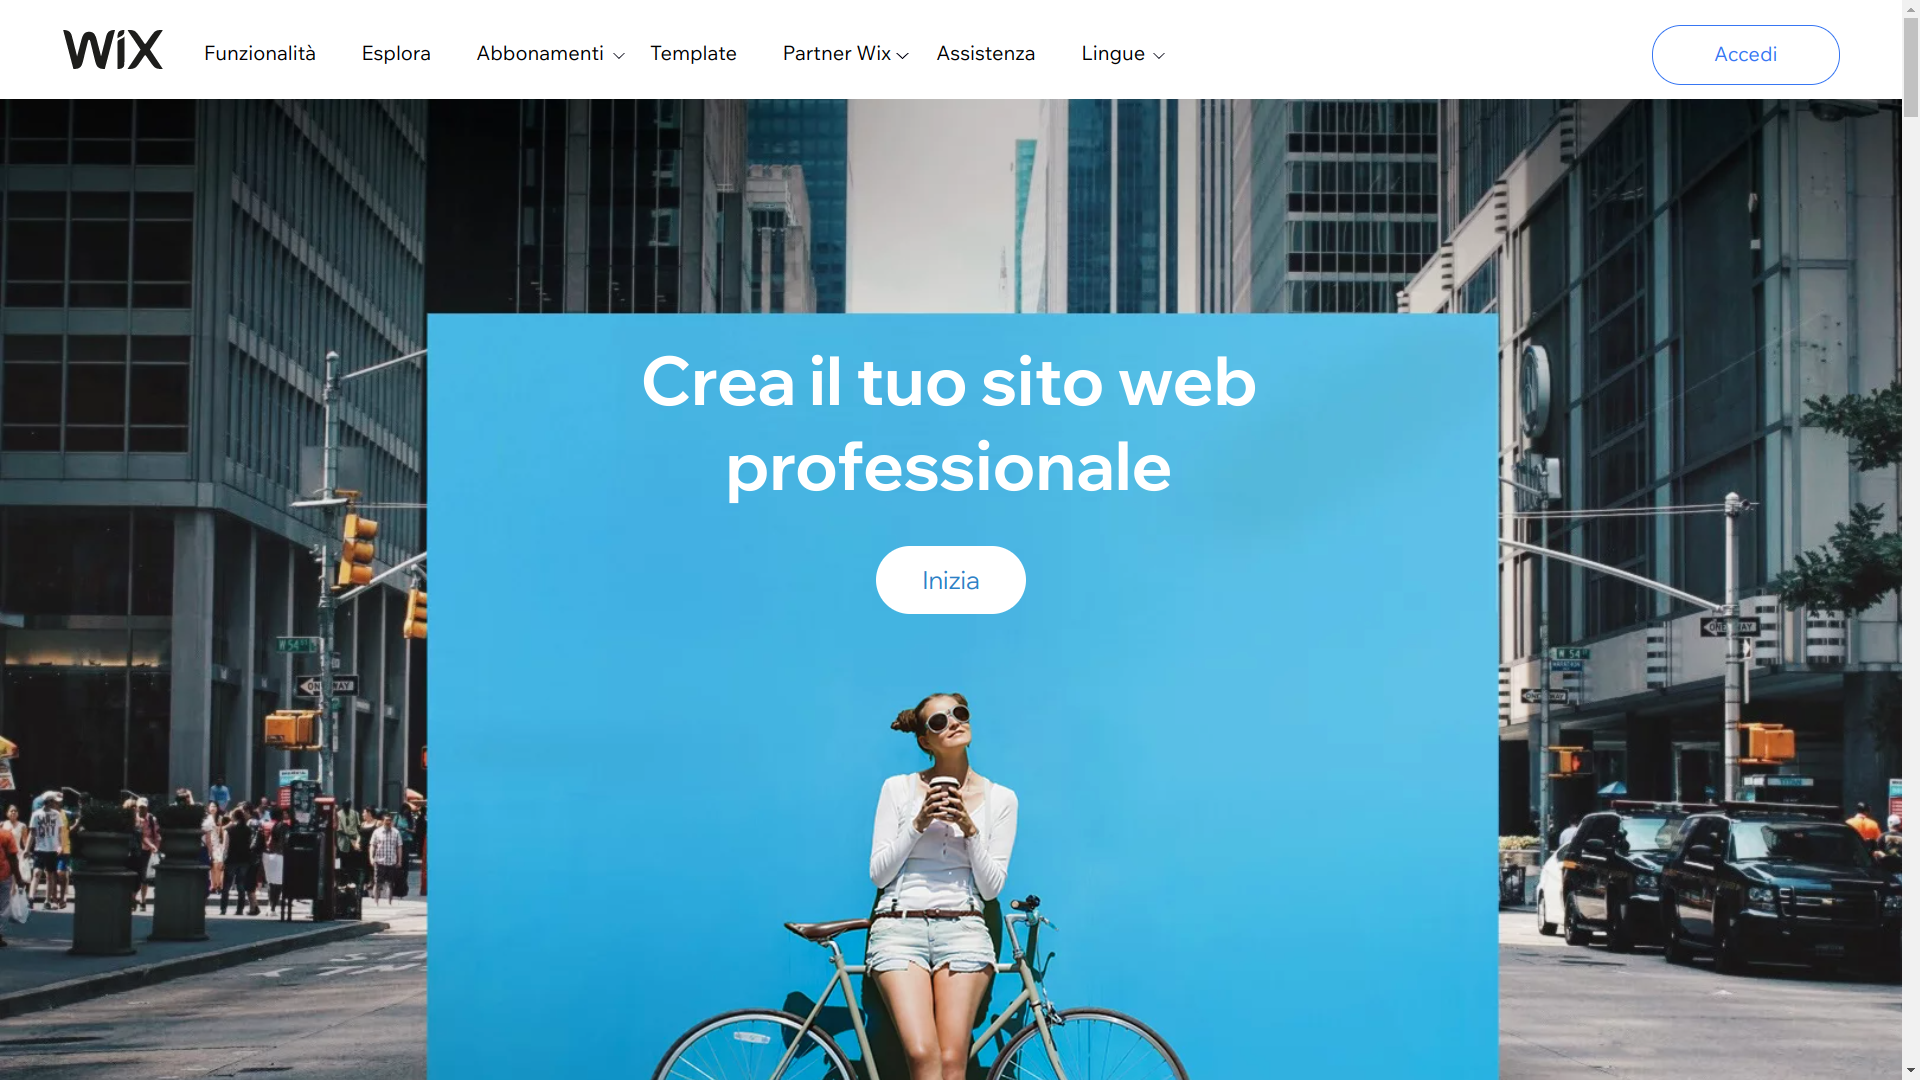
\includegraphics[width=1\textwidth]{img/homepage-01.png}
  \caption{Homepage (pt. 1)}
  \label{fig:homepage-01}
\end{figure}

Proseguendo con il primo scroll, la figura \ref{fig:homepage-02}
mostra la seconda schermata del sito web. Vi è un titolo molto
evocativo sulla sinistra ma comunque poco informativo, mentre il
paragrafo descrive meglio l'obiettivo di \wix{}. Il link
\textit{Inizia} porta ancora una volta alla pagina di registrazione
piuttosto che fornire altre informazioni. Per queste dobbiamo
scrollare.

\begin{figure}[H]
  \centering
  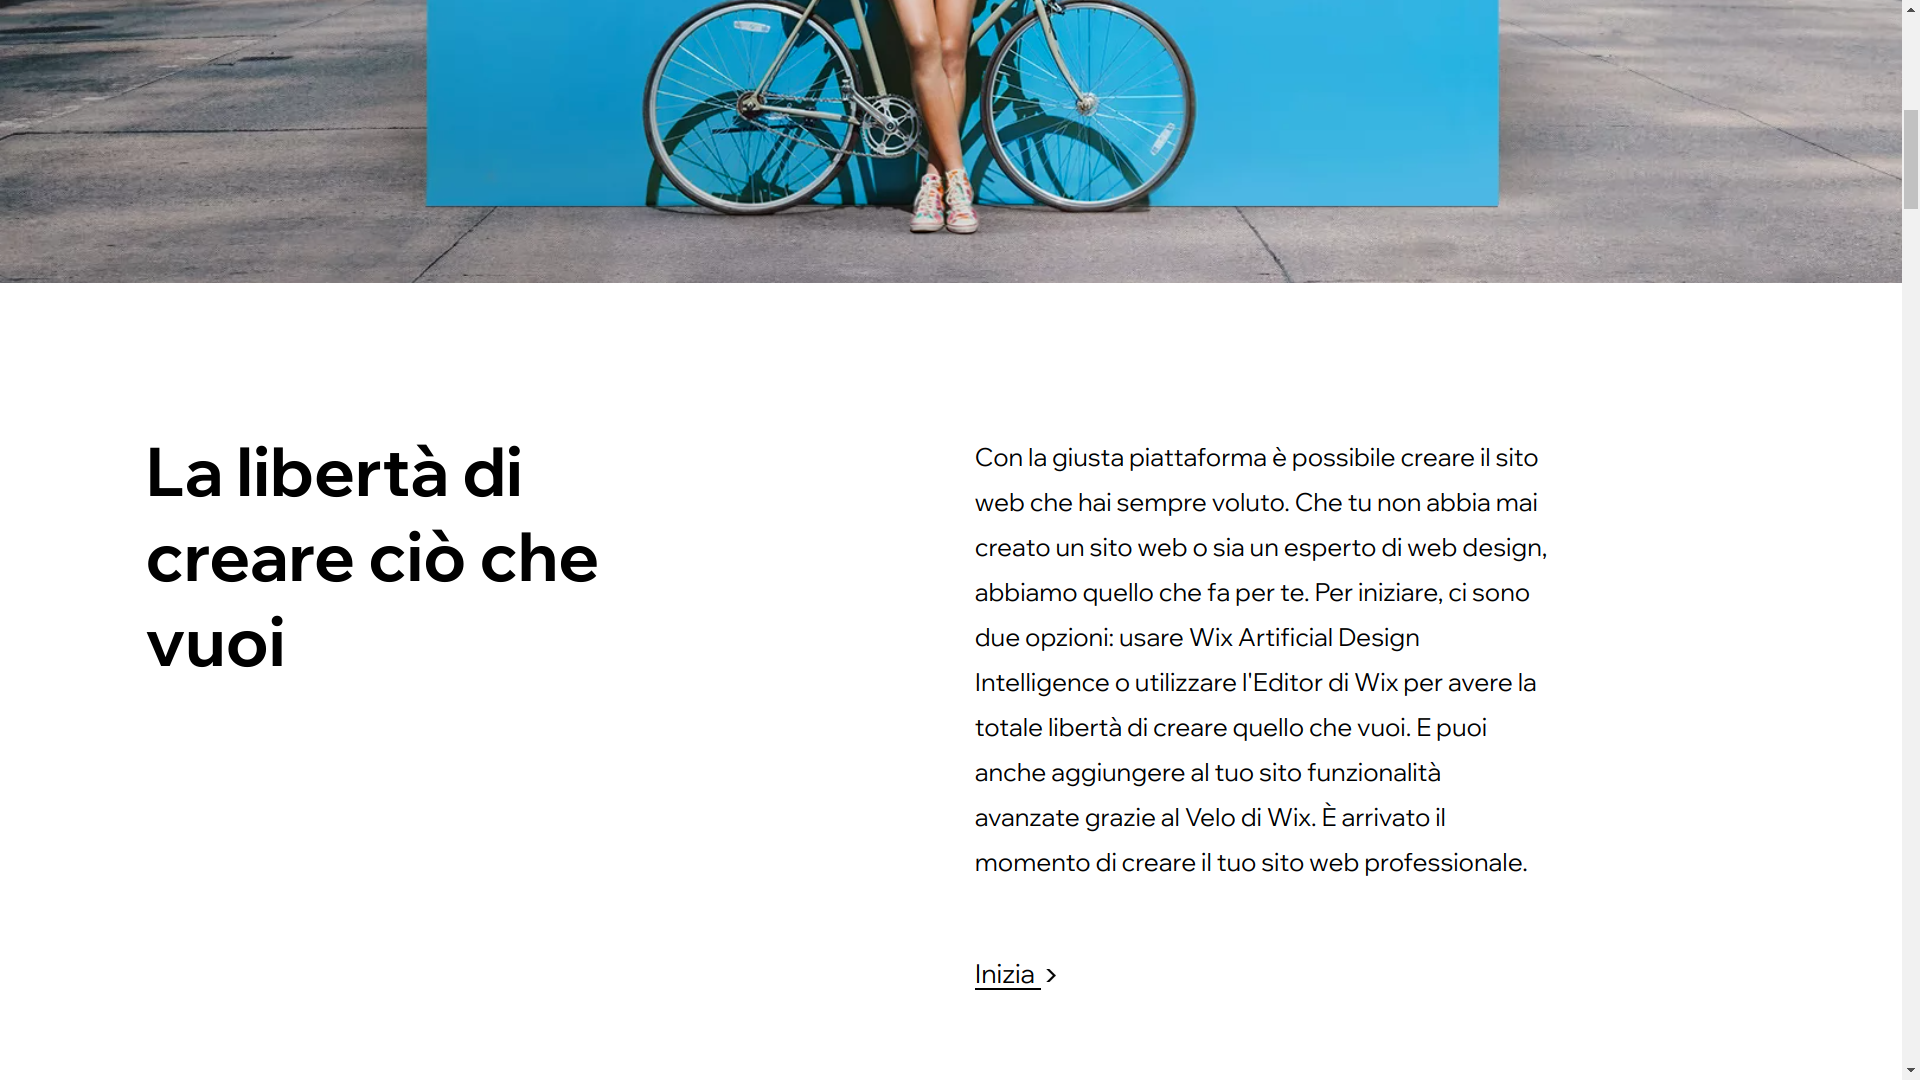
\includegraphics[width=1\textwidth]{img/homepage-02.png}
  \caption{Homepage (pt. 2)}
  \label{fig:homepage-02}
\end{figure}

Le immagini \ref{fig:homepage-03}, \ref{fig:homepage-04} e
\ref{fig:homepage-05} raffigurano le schermate della homepage dove vi
sono alcune informazioni sul prodotto presentato. I titoli non sono
del tutto chiari, ad esempio ``Velo'' e ``Wix ADI'' non restituiscono
all'utente un feedback immediato su quello che andrà a leggere, anche
se poi sono presenti dei sottotitoli indicano meglio di cosa si sta
parlando. 

Queste tre schermate, pur essendo molto belle visivamente sprecano non
poco spazio nell'illustrare le funzionalità del prodotto: le immagini
non sono sfruttate al massimo per enfatizzare il testo in quanto i box
separano concettualmente testo dall'immagine.

\begin{figure}[H]
  \centering
  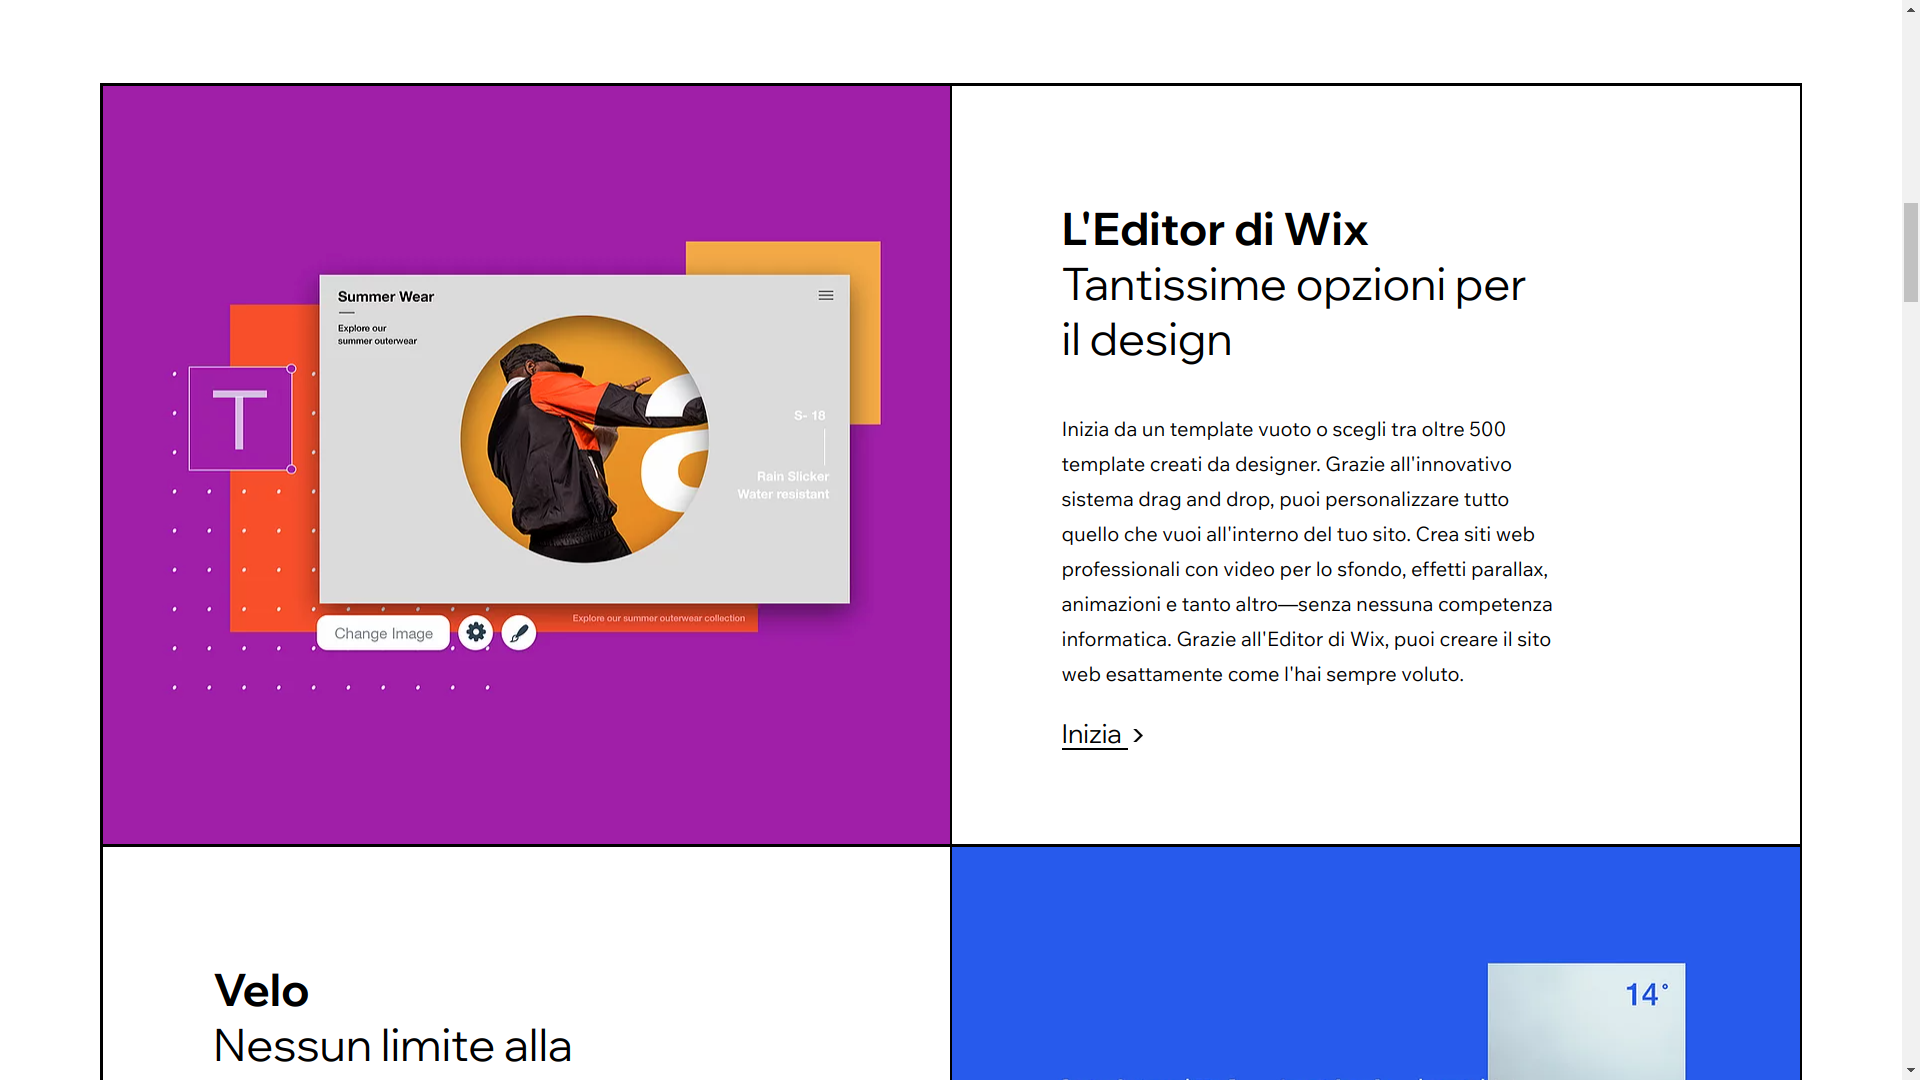
\includegraphics[width=1\textwidth]{img/homepage-03.png}
  \caption{Homepage (pt. 3)}
  \label{fig:homepage-03}
\end{figure}

\begin{figure}[H]
  \centering
  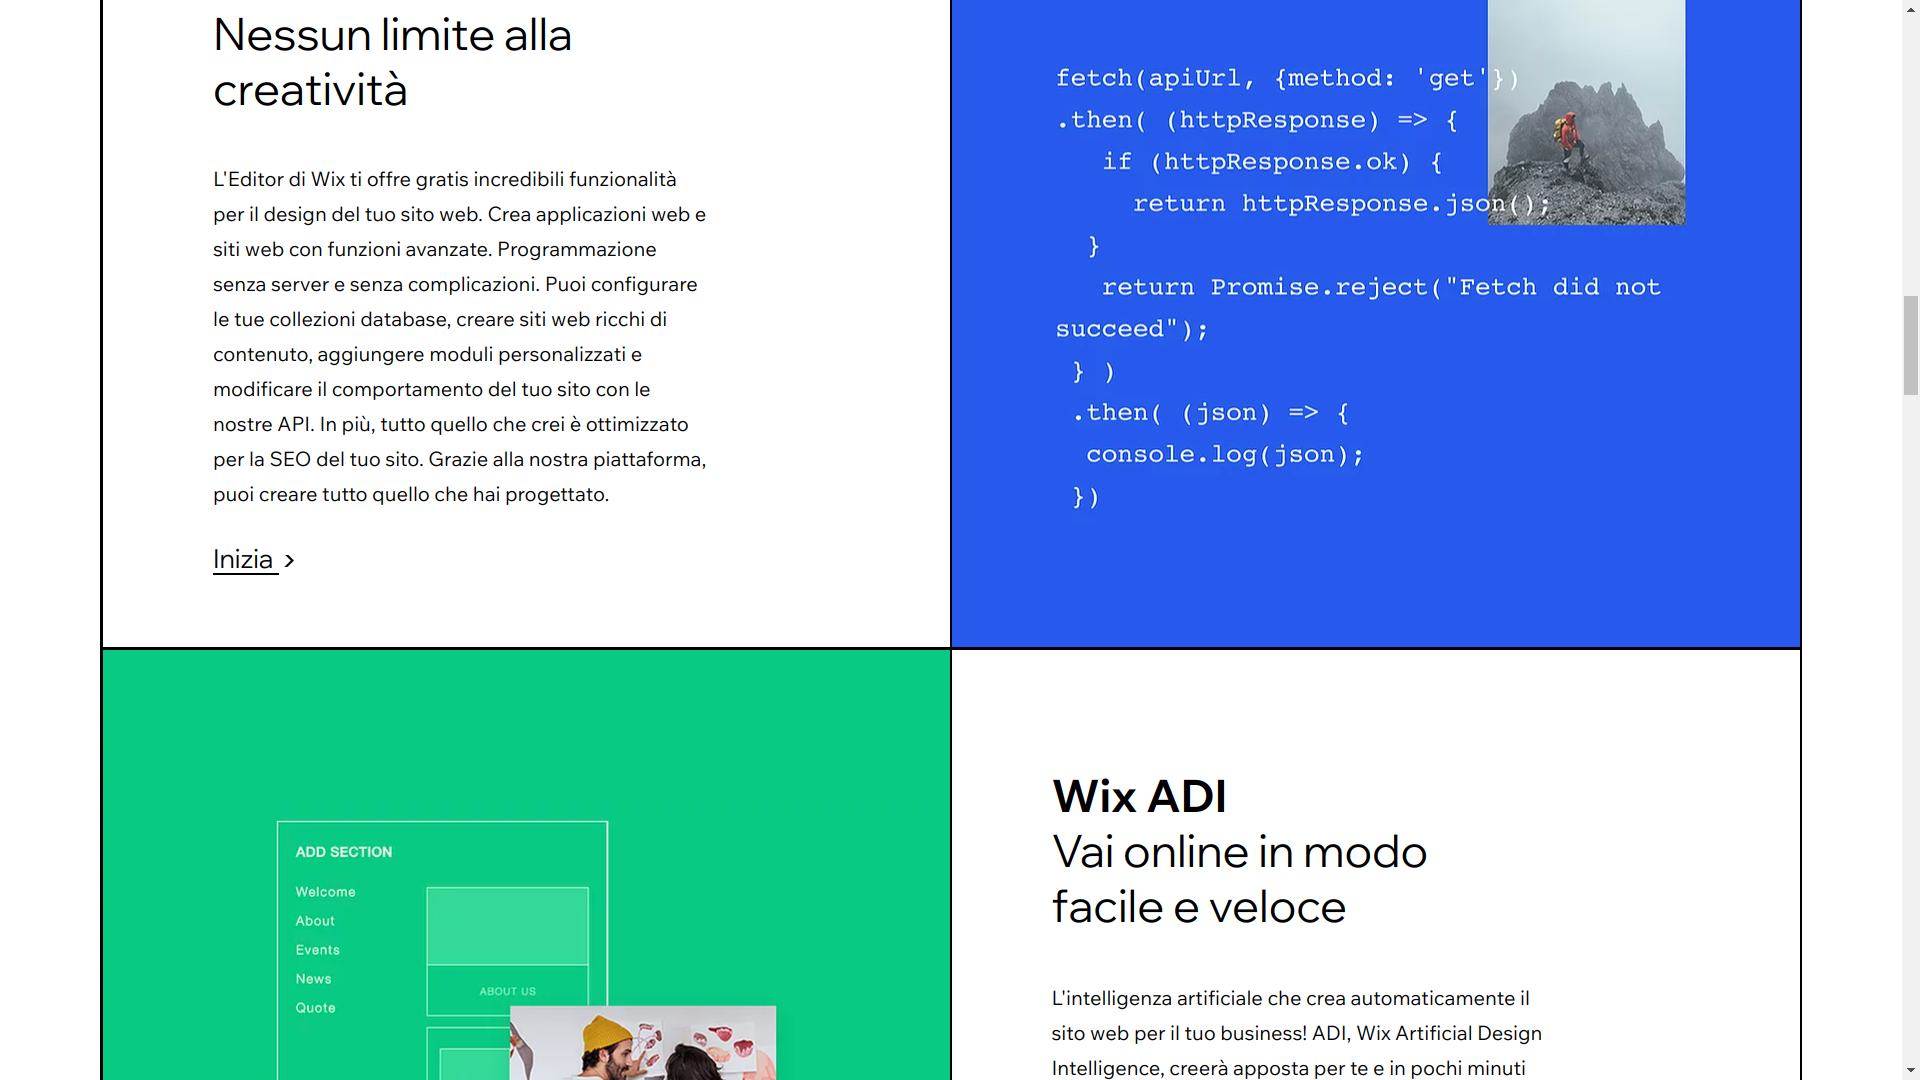
\includegraphics[width=1\textwidth]{img/homepage-04.png}
  \caption{Homepage (pt. 4)}
  \label{fig:homepage-04}
\end{figure}

\begin{figure}[H]
  \centering
  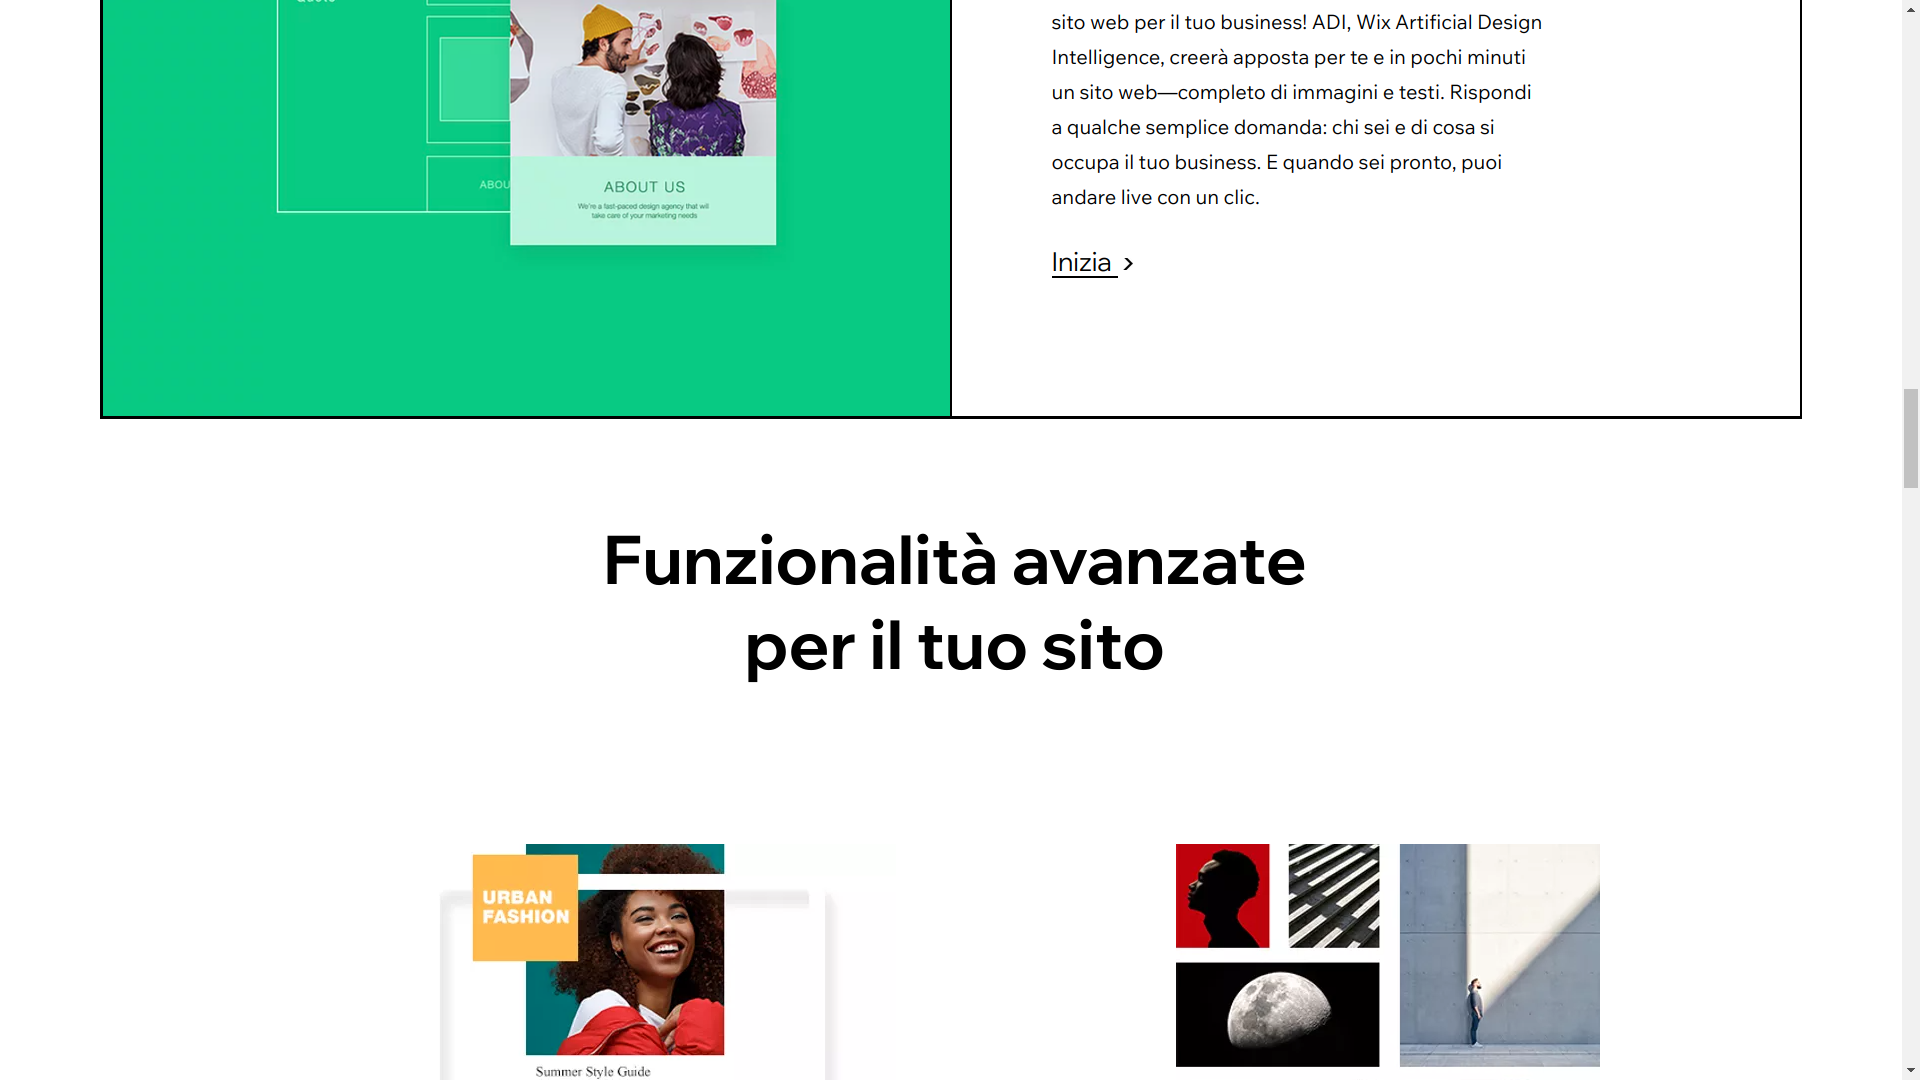
\includegraphics[width=1\textwidth]{img/homepage-05.png}
  \caption{Homepage (pt. 5)}
  \label{fig:homepage-05}
\end{figure}

La percentuale di utenti che continua ad essere presenti sul sito web
dopo quattro scroll è drasticamente ridotta, ma di fatto sono stati
presentati pochi contenuti, infatti il sito web continua con le
schermate \ref{fig:homepage-06} e \ref{fig:homepage-07}. In queste due
schermate vengono presentate altre funzionalità (avanzate) dello
strumento. Questi paragrafi sono concisi ed efficaci, inoltre sono
supportati da titoli che enfatizzano bene il concetto descritto. Anche
in questo caso però si spreca molto spazio con le immagini. La
presentazione delle caratteristiche inoltre è strutturata secondo uno
schema a griglia, e anche se gli elementi a schermo sono pochi, questa
distribuzione dei contenuti può generare confusione nell'utente dovuta
all'effetto \textit{random walk}.

\begin{figure}[H]
  \centering
  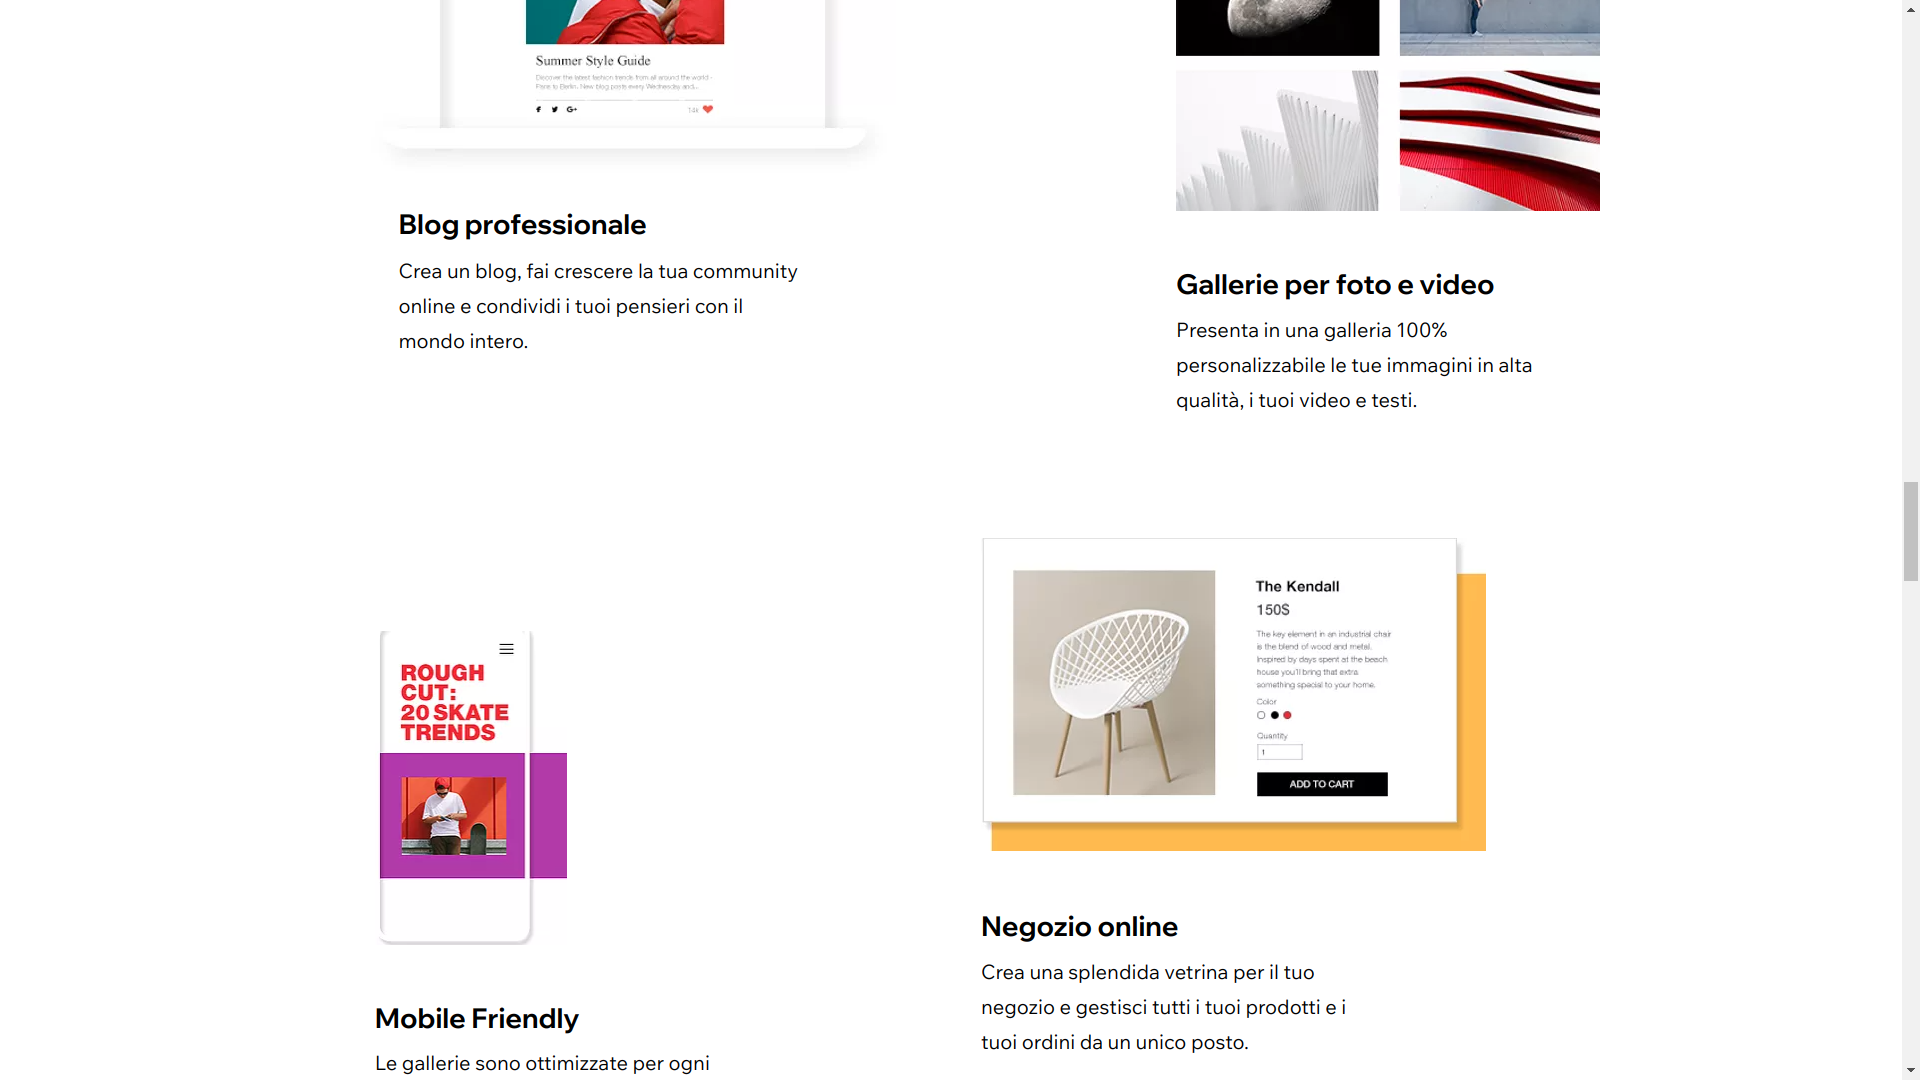
\includegraphics[width=1\textwidth]{img/homepage-06.png}
  \caption{Homepage (pt. 6)}
  \label{fig:homepage-06}
\end{figure}

\begin{figure}[H]
  \centering
  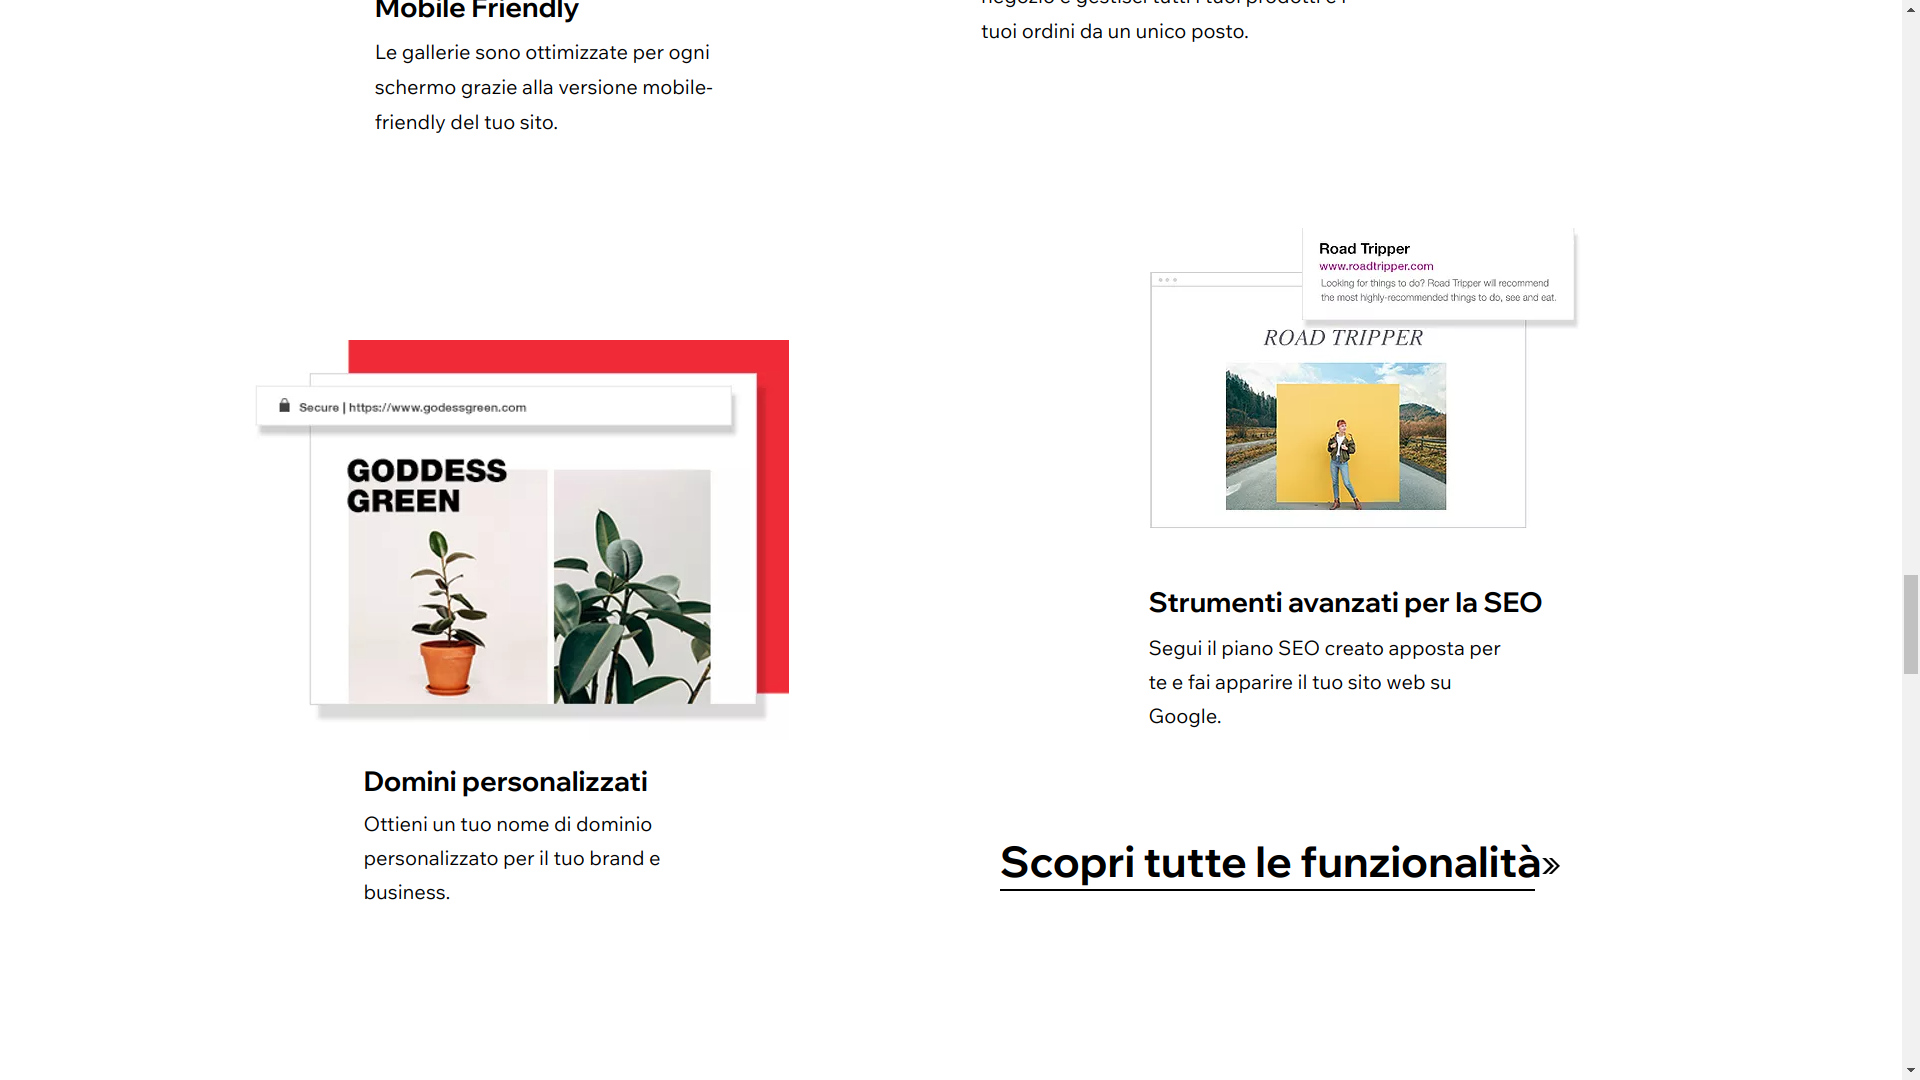
\includegraphics[width=1\textwidth]{img/homepage-07.png}
  \caption{Homepage (pt. 7)}
  \label{fig:homepage-07}
\end{figure}

Le schermate \ref{fig:homepage-08} e \ref{fig:homepage-09} illustrano
altre informazioni su \wix{}. In particolare viene esplicitata
l'utenza target, ovvero utenti con o senza conoscenza informatica e il
perché \wix{} è lo strumento da scegliere per costruire un sito web.

\begin{figure}[H]
  \centering
  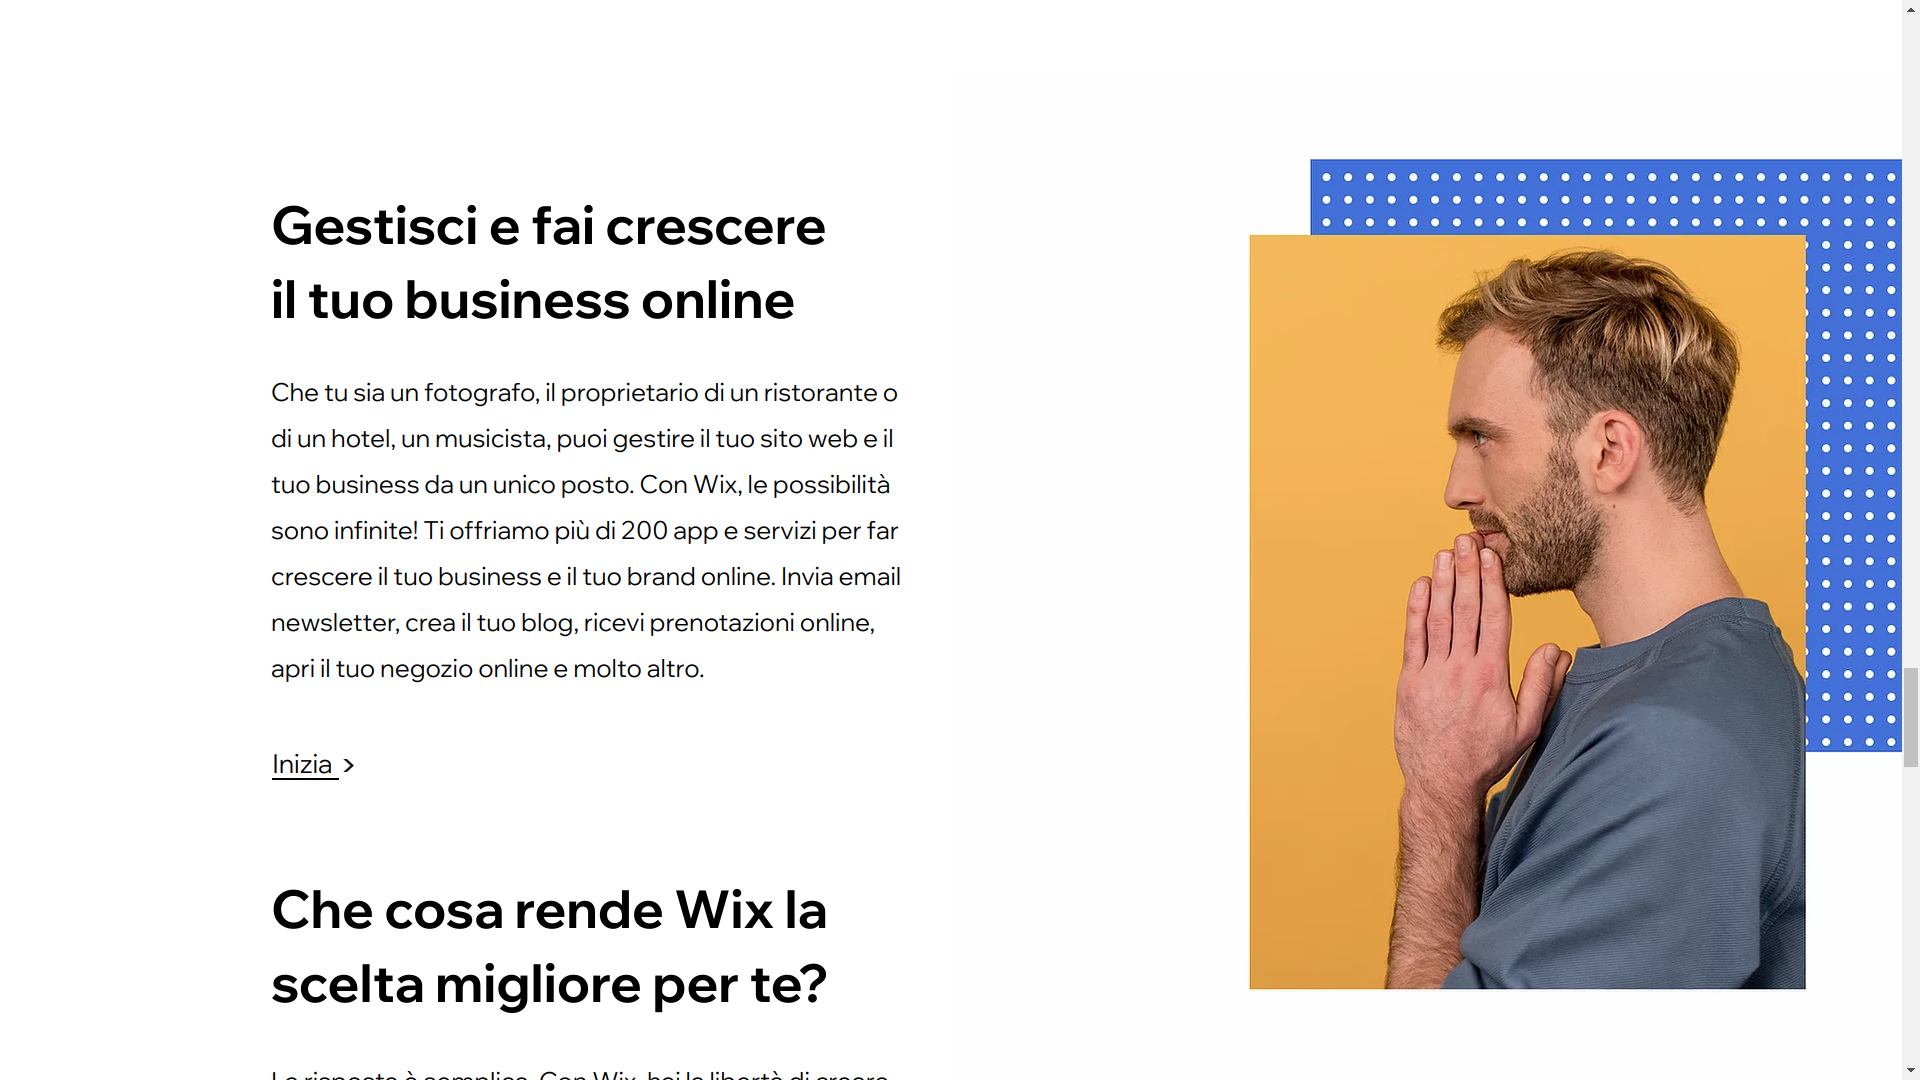
\includegraphics[width=1\textwidth]{img/homepage-08.png}
  \caption{Homepage (pt. 8)}
  \label{fig:homepage-08}
\end{figure}

\begin{figure}[H]
  \centering
  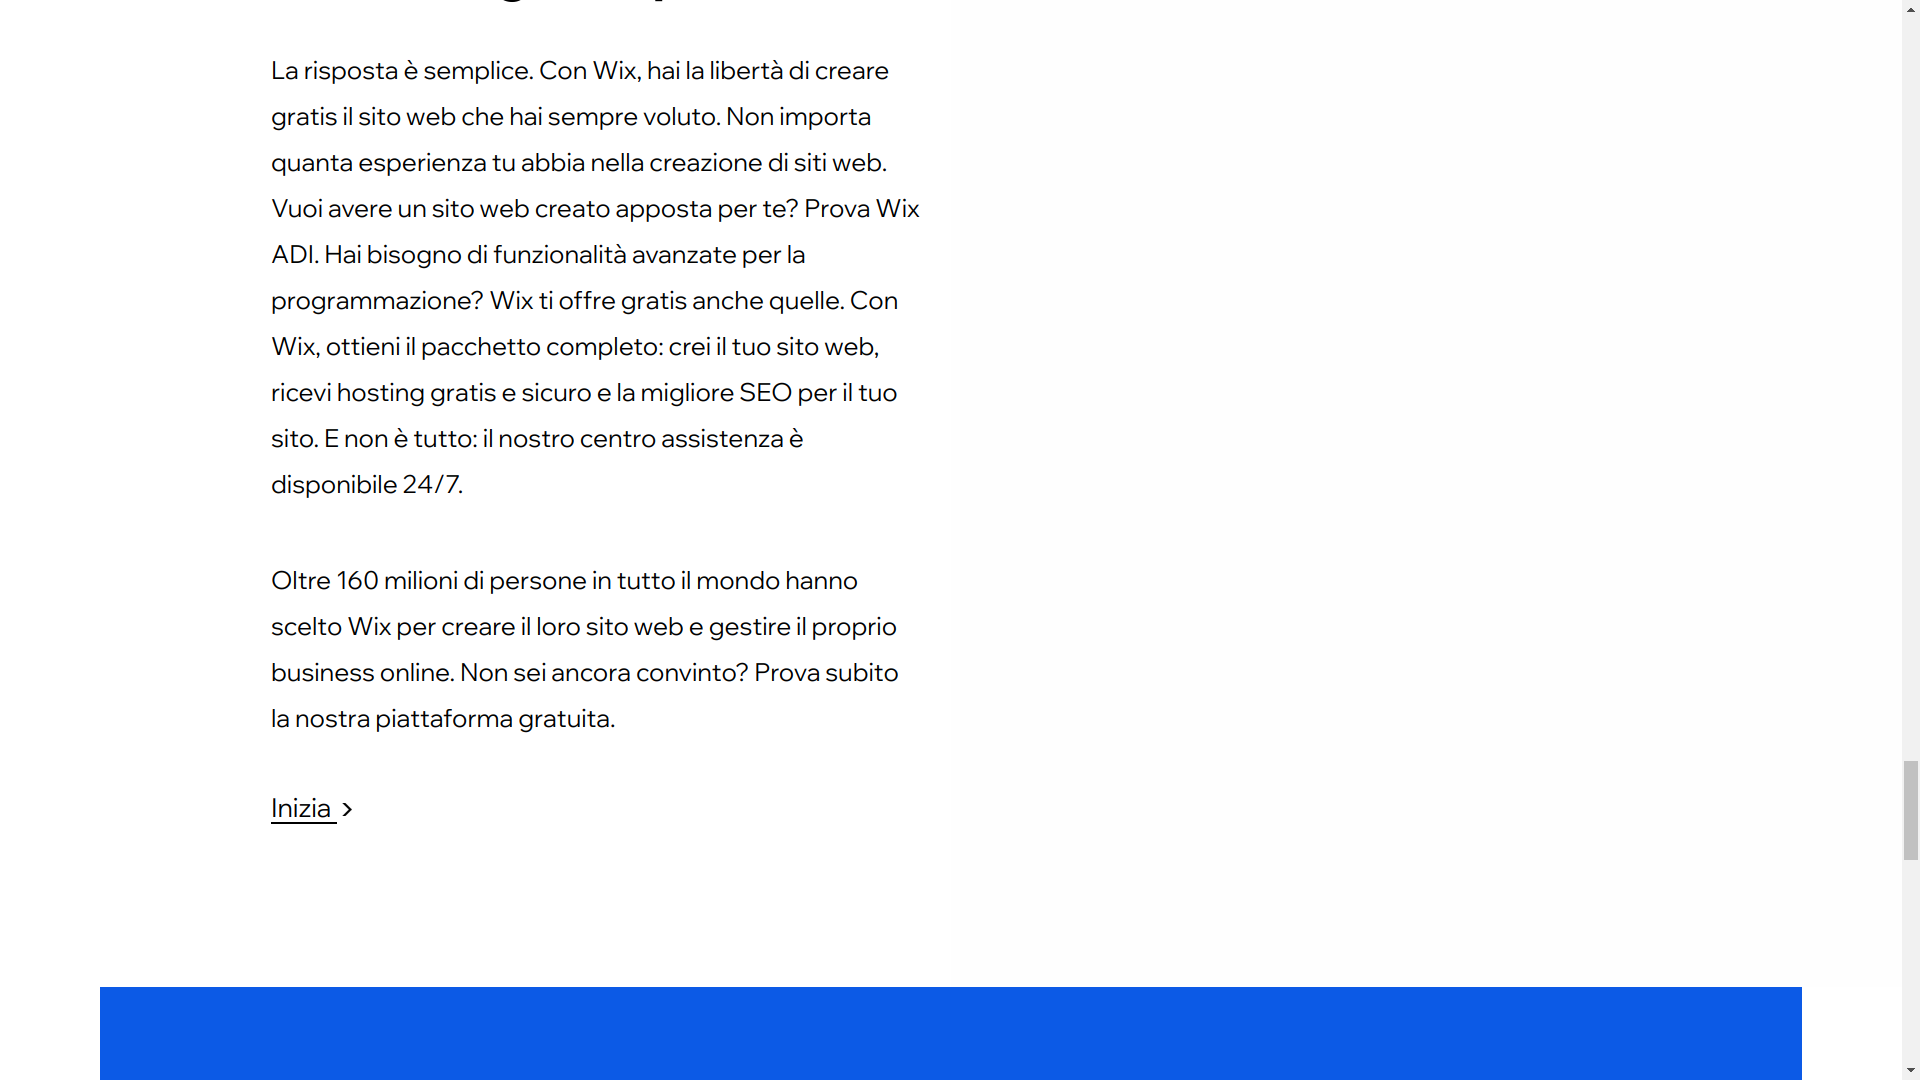
\includegraphics[width=1\textwidth]{img/homepage-09.png}
  \caption{Homepage (pt. 9)}
  \label{fig:homepage-09}
\end{figure}

La scheramata \ref{fig:homepage-10} mostra passo per passo gli step da
seguire per ``Creare gratis un sito web'', come recita il titolo.

\begin{figure}[H]
  \centering
  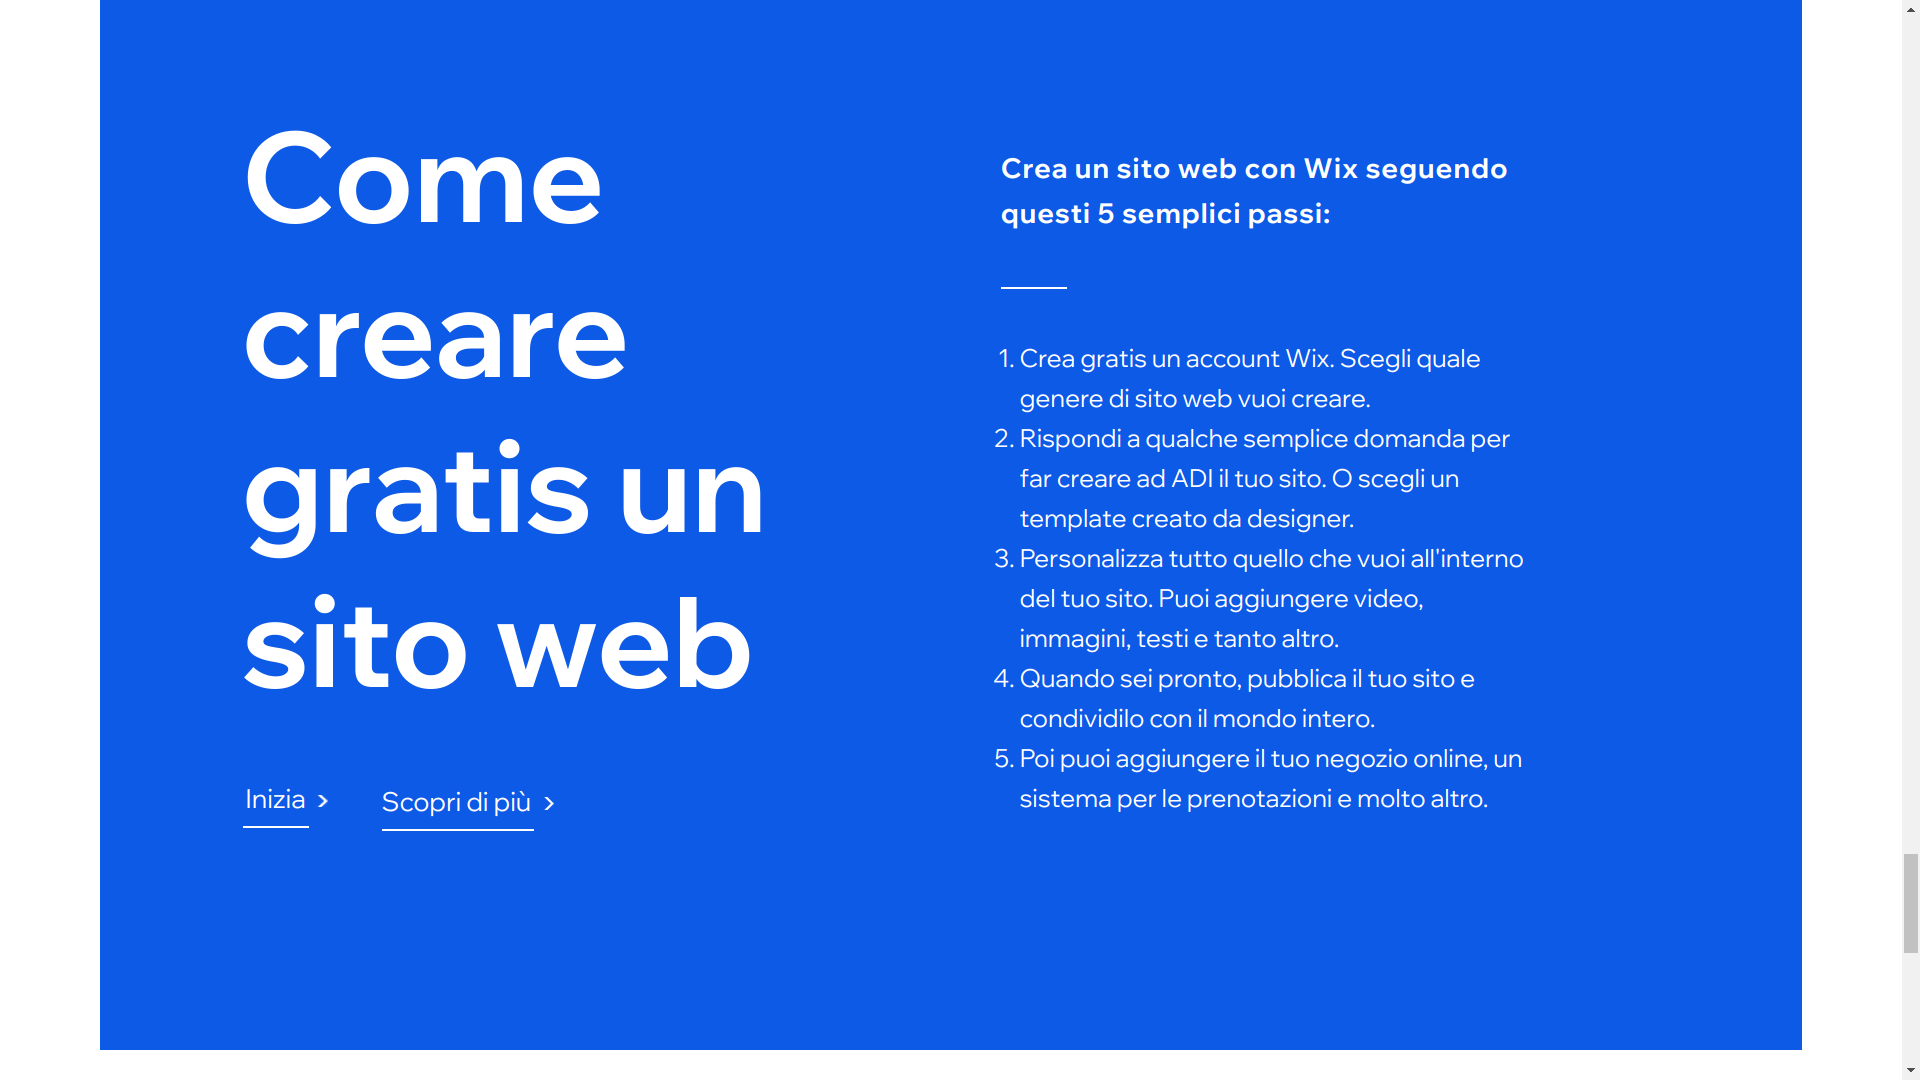
\includegraphics[width=1\textwidth]{img/homepage-10.png}
  \caption{Homepage (pt. 10)}
  \label{fig:homepage-10}
\end{figure}

Con la schermata \ref{fig:homepage-11} finalmente si conclude la
homepage. Sono forniti diversi link a prodotti correlati, informazioni
sull'azienda e riferimenti al supporto.

\begin{figure}[H]
  \centering
  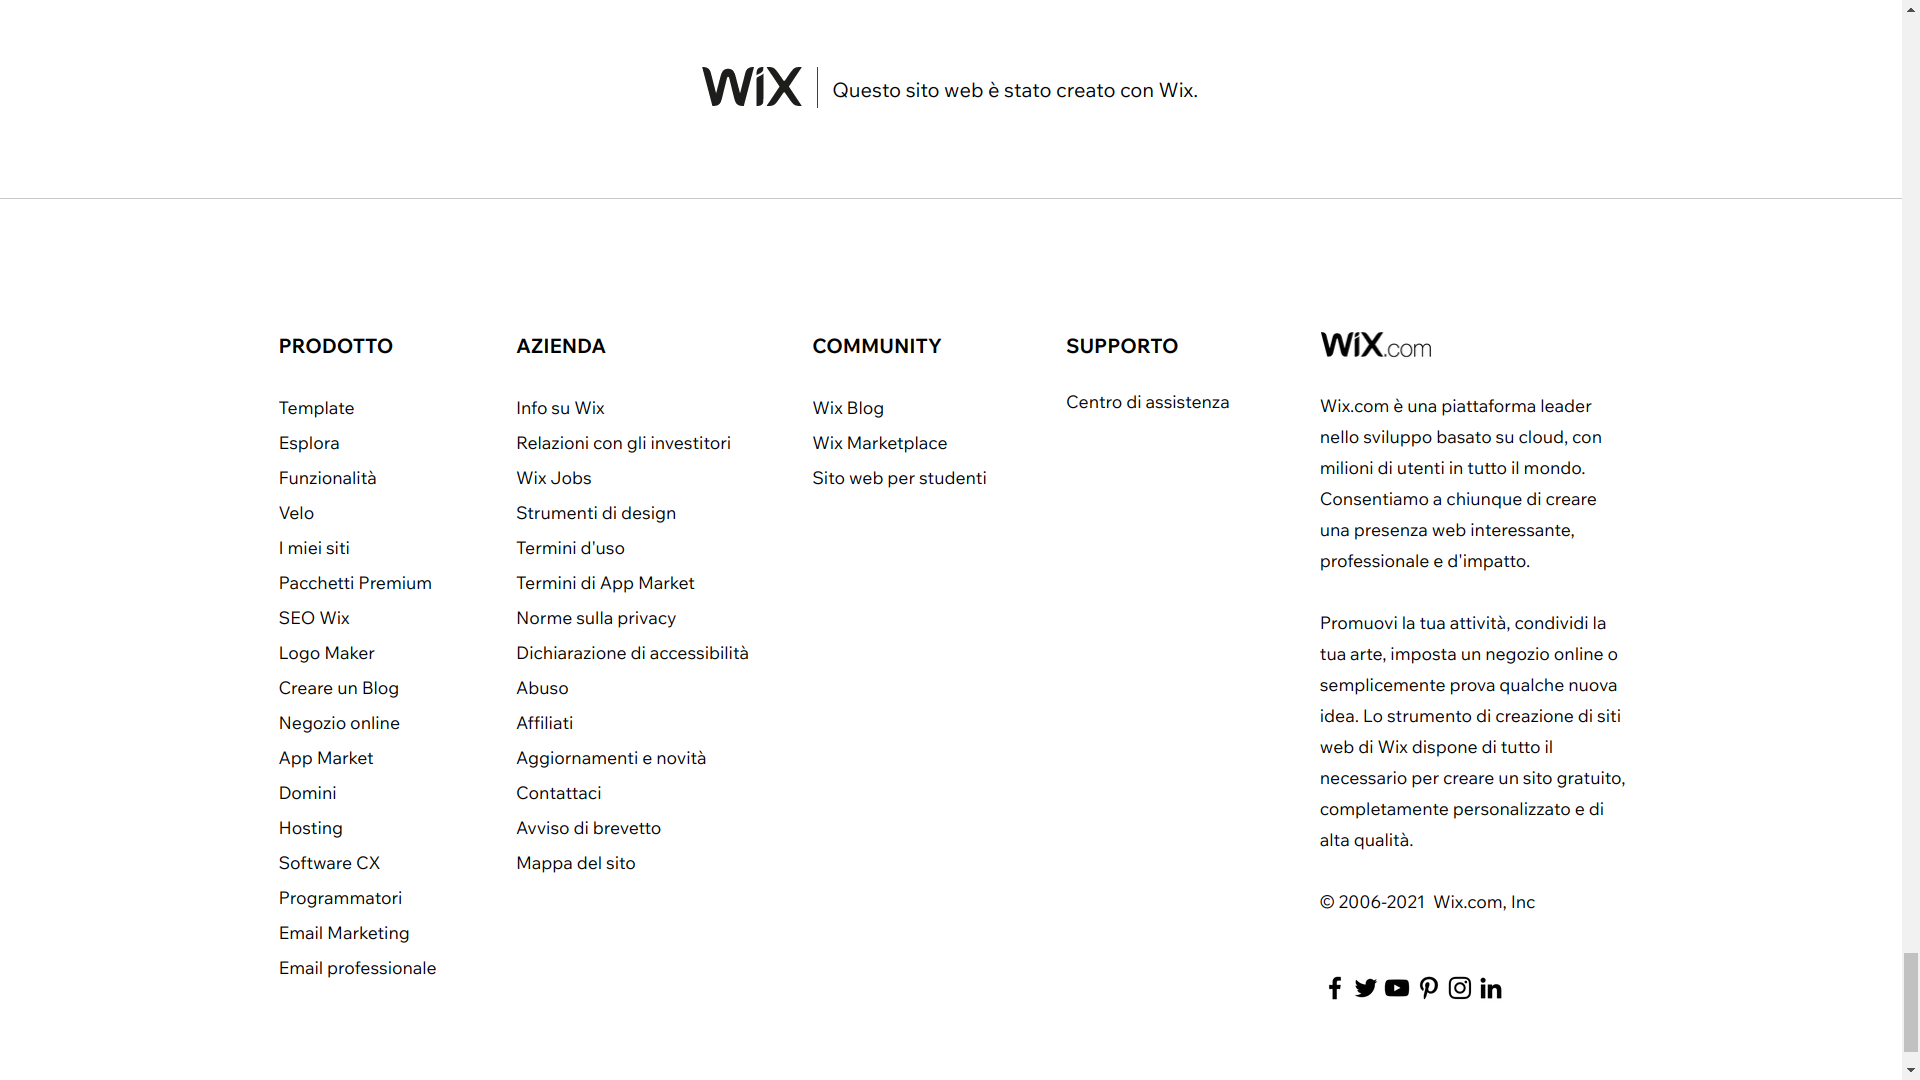
\includegraphics[width=1\textwidth]{img/homepage-11.png}
  \caption{Homepage (pt. 11)}
  \label{fig:homepage-11}
\end{figure}

\subsection{The Six Ws}
\label{subsec:homepage-the-six-ws}

Analizziamo gli assi informativi della homepage.

\begin{itemize}
  \item \textbf{Where?} \textit{In quale sito web mi trovo?}
    L'immagine \ref{fig:homepage-01} mostra ciò che vedrebbe un utente
    capitato nel sito web \wix{}. Purtroppo la prima schermata non è
    molto informativa e l'utente cercherebbe di capire dove si trova
    principalmente dal logo e dal titolo della pagina. Il logo non è
    informativo sul prodotto, e anche se \wix{} è abbastanza famoso
    anche grazie alla pubblicità, sono necessarie altre
    informazioni. Il titolo della pagina recita ``Crea il tuo sito web
    professionale''. Da qui l'utente può dedurre che \wixcom{}
    permette di creare siti web, ma in che modo lo fa? Ci sono dei
    professionisti che realizzano il sito oppure è l'utente che se lo
    può costruire? Per rispondere a questa domanda bisogna
    scrollare. In figura \ref{fig:homepage-02} (seconda schermata) si
    trova la risposta a questa domanda: \wix{} è una piattaforma per
    creare siti web.

  \item \textbf{Who?} \textit{Chi c'è dietro a questo sito?} Questa
    informazione non è immediata e l'unico modo per rispondere
    esplicitamente alla domanda è arrivare al footer della homepage
    (figura \ref{fig:homepage-11}).

  \item \textbf{Why?} \textit{Quali benefici offre il sito?} Alcune
    informazioni per rispondere a questa domanda sono accessibili dopo
    un primo scroll (figura \ref{fig:homepage-02}) dal paragrafo
    descrittivo, ma la risposta viene data principalmente dalle
    schermata in figura \ref{fig:homepage-08} e \ref{fig:homepage-09}
    dopo ben sette scroll. Il titolo ``Che cosa rende Wix la scelta
    migliore per te?'' è significativo in questa sezione, perché
    cattura in maniera esplicita la domanda dell'asse.

  \item \textbf{What?} \textit{Cosa viene offerto da questo sito?} La
    risposta viene parzialmente coperta dal titolo nella prima
    schermata della homepage (figura \ref{fig:homepage-01}), ma il
    realtà la maggior parte delle informazioni vengono fornite con
    diversi scroll successivi. La schemata \ref{fig:homepage-02}
    mostra una prima descrizione di massima del prodotto. Le schemate
    riportate in figura \ref{fig:homepage-03}, \ref{fig:homepage-03} e
    \ref{fig:homepage-05} illustrano le principali funzionalità di
    \wix{}, mentre le caratteristiche avanzate dello strumento sono
    discusse dalle schemate in figura \ref{fig:homepage-06} e
    \ref{fig:homepage-07}.

  \item \textbf{When?} \textit{Quali sono le ultime novità del sito?}
    La risposta nella homepage non è fornita in alcun modo e nel menu
    principale non ci sono riferimenti ad altre pagine che possano
    presentare novità. L'unica pagina che illustra alcune novita
    rispetto a \wix{} è \textit{Wix Blog}, accessibile dal footer
    (figura \ref{fig:homepage-11}).

  \item \textbf{How?} \textit{Come accedo alle funzionalità presentate
    dal sito?} La risposta a questa domanda è interamente fornita
    dalla schermata in figura \ref{fig:homepage-10}. Anche qui il
    titolo ``Come creare gratis un sito web'' cattura a pieno la
    domanda. Inoltre, in questo caso si frutta anche il trucco della
    parola gratis, che genera una sensazione di piacere per l'utente.  
\end{itemize}

\section{Pagina interna: Dominio}
\label{sec:secondary-page-analysis}

Ho scelto di analizzare la pagina ``Dominio'' come pagina interna di
\wix{}, accessibile tramite l'URL
\url{https://it.wix.com/domain/names}. Deciso di discutere questa
pagina in quanto ritengo che un motore di ricerca possa facilmente
consigliare questa pagina ad un utente che sta cercando informazioni
sulla creazione di un dominio/sito web.

La pagina web dovrà quindi essere in grado di fornire le informazioni
che l'utente sta cercando e, se l'obiettivo va oltre quello meramente
informativo, mantenere l'utente sul sito per presentare e possibilmente
vendere il proprio prodotto.

\subsection{Descrizione generale}
\label{subsec:internalpage-description}

La pagina web, illustrata in figura \ref{fig:domain-01}, si apre con
un'immagine molto grande che occupa buona parte dello schermo. Anche
qui l'entry point del sito è ben definito: il logo in alto a
sinistra. Ci vengono poi presentate le prime informazioni grazie al
titolo e, soprattutto, al sottotitolo. A questo punto però l'utente
non ha ancora capito se è in una pagina informativa o più di vendita
di prodotto, ed è obbligato a continuare la navigazione per conoscere
altre informazioni. La parte terminale della pagina spiega come
ottnere un nuovo dominio e sfrutta diversi accorgimenti sul testo:
titolo del paragrafo con font-size più grande, sottotitolo
eviadenziato in grassetto e poi qualche riga di testo.

\begin{figure}[H]
  \centering
  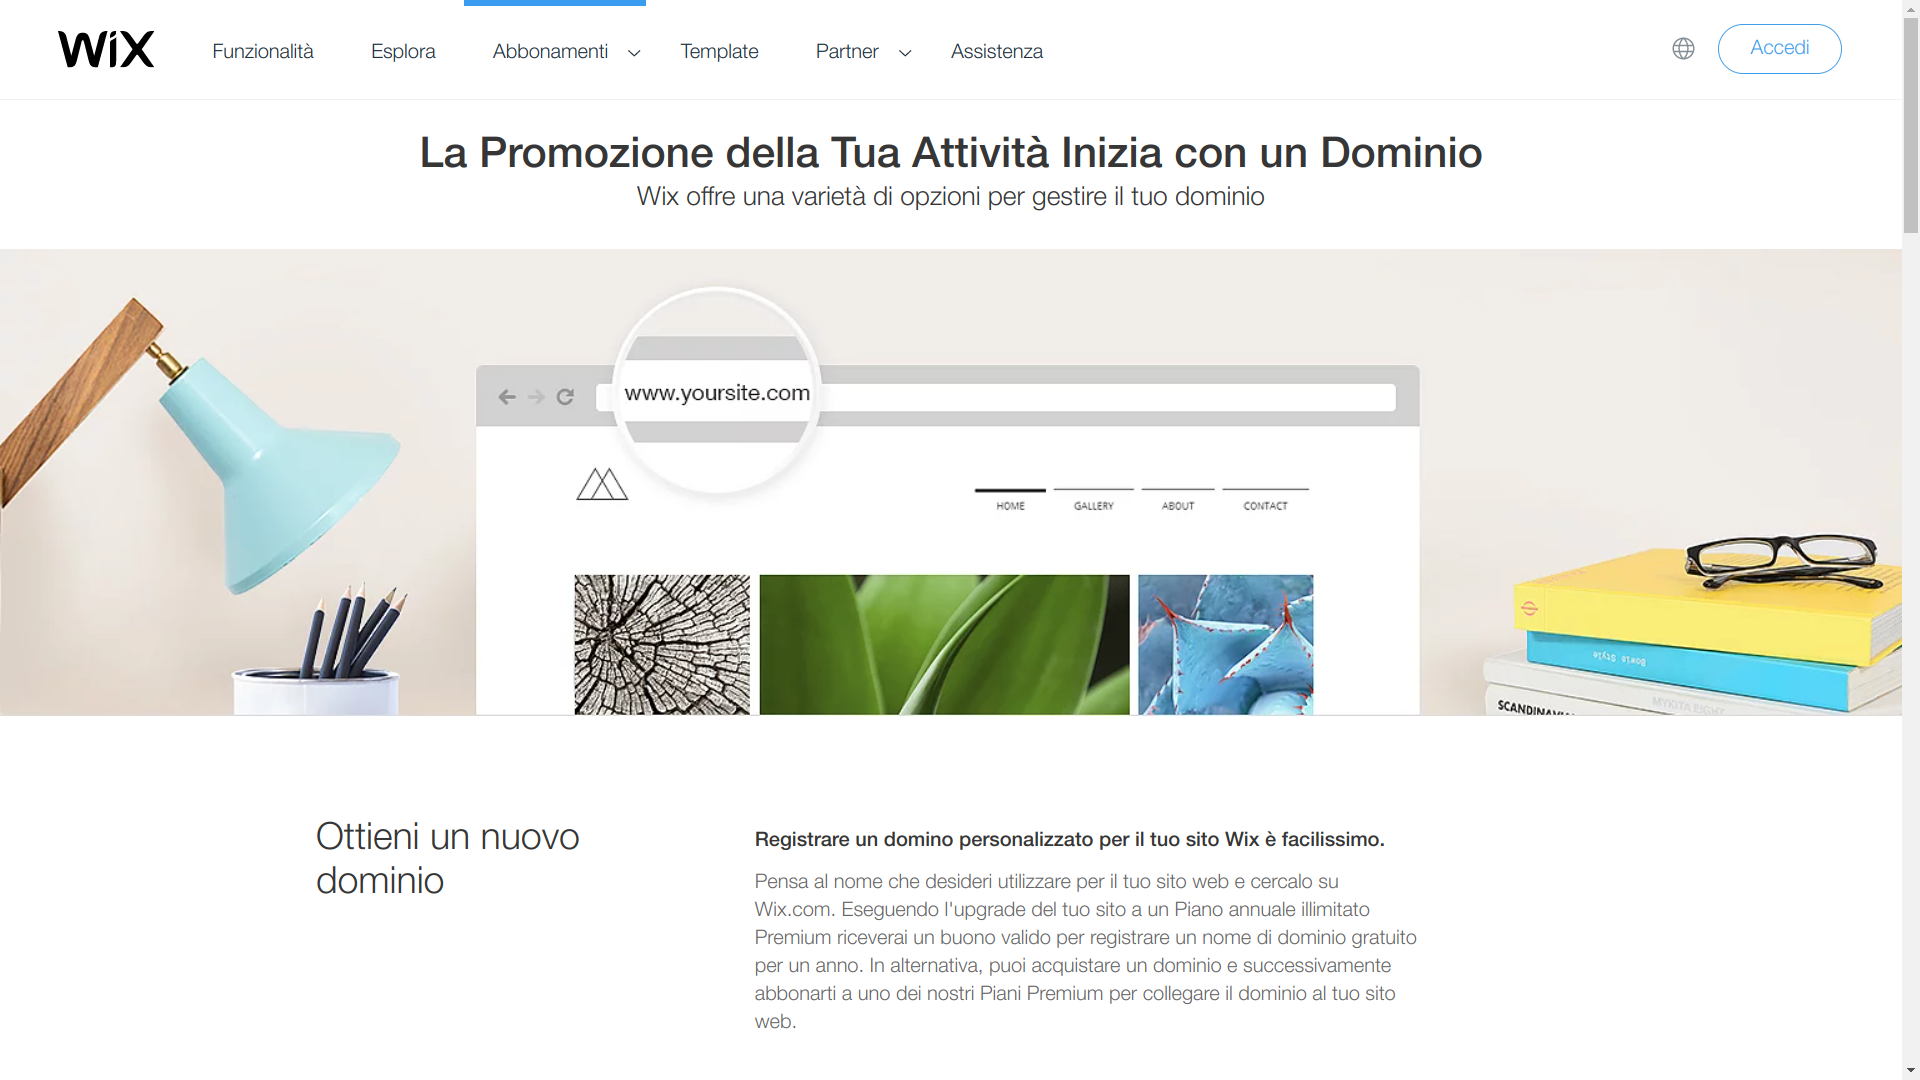
\includegraphics[width=1\textwidth]{img/domain-01.png}
  \caption{Dominio (pt. 1)}
  \label{fig:domain-01}
\end{figure}

Continuando con il primo scroll l'utente viene sottoposto alle
informazioni riportate in figura \ref{fig:domain-02}. Qui vengono
forniti dettagli di carattere informativo che sono sicuramente utili
per un utente (quasi) inserpeto. In questo paragrafo \wix{} mette in
atto anche la tecnica dell'honeypot: viene fornito contenuto
appetibile agli altri siti che, sperabilmente, linkeranno la pagina
per fornire informazioni su cosa è un dominio. Anche qui, sono
applicate tecniche sul testo che favoriscono la lettura.

\begin{figure}[H]
  \centering
  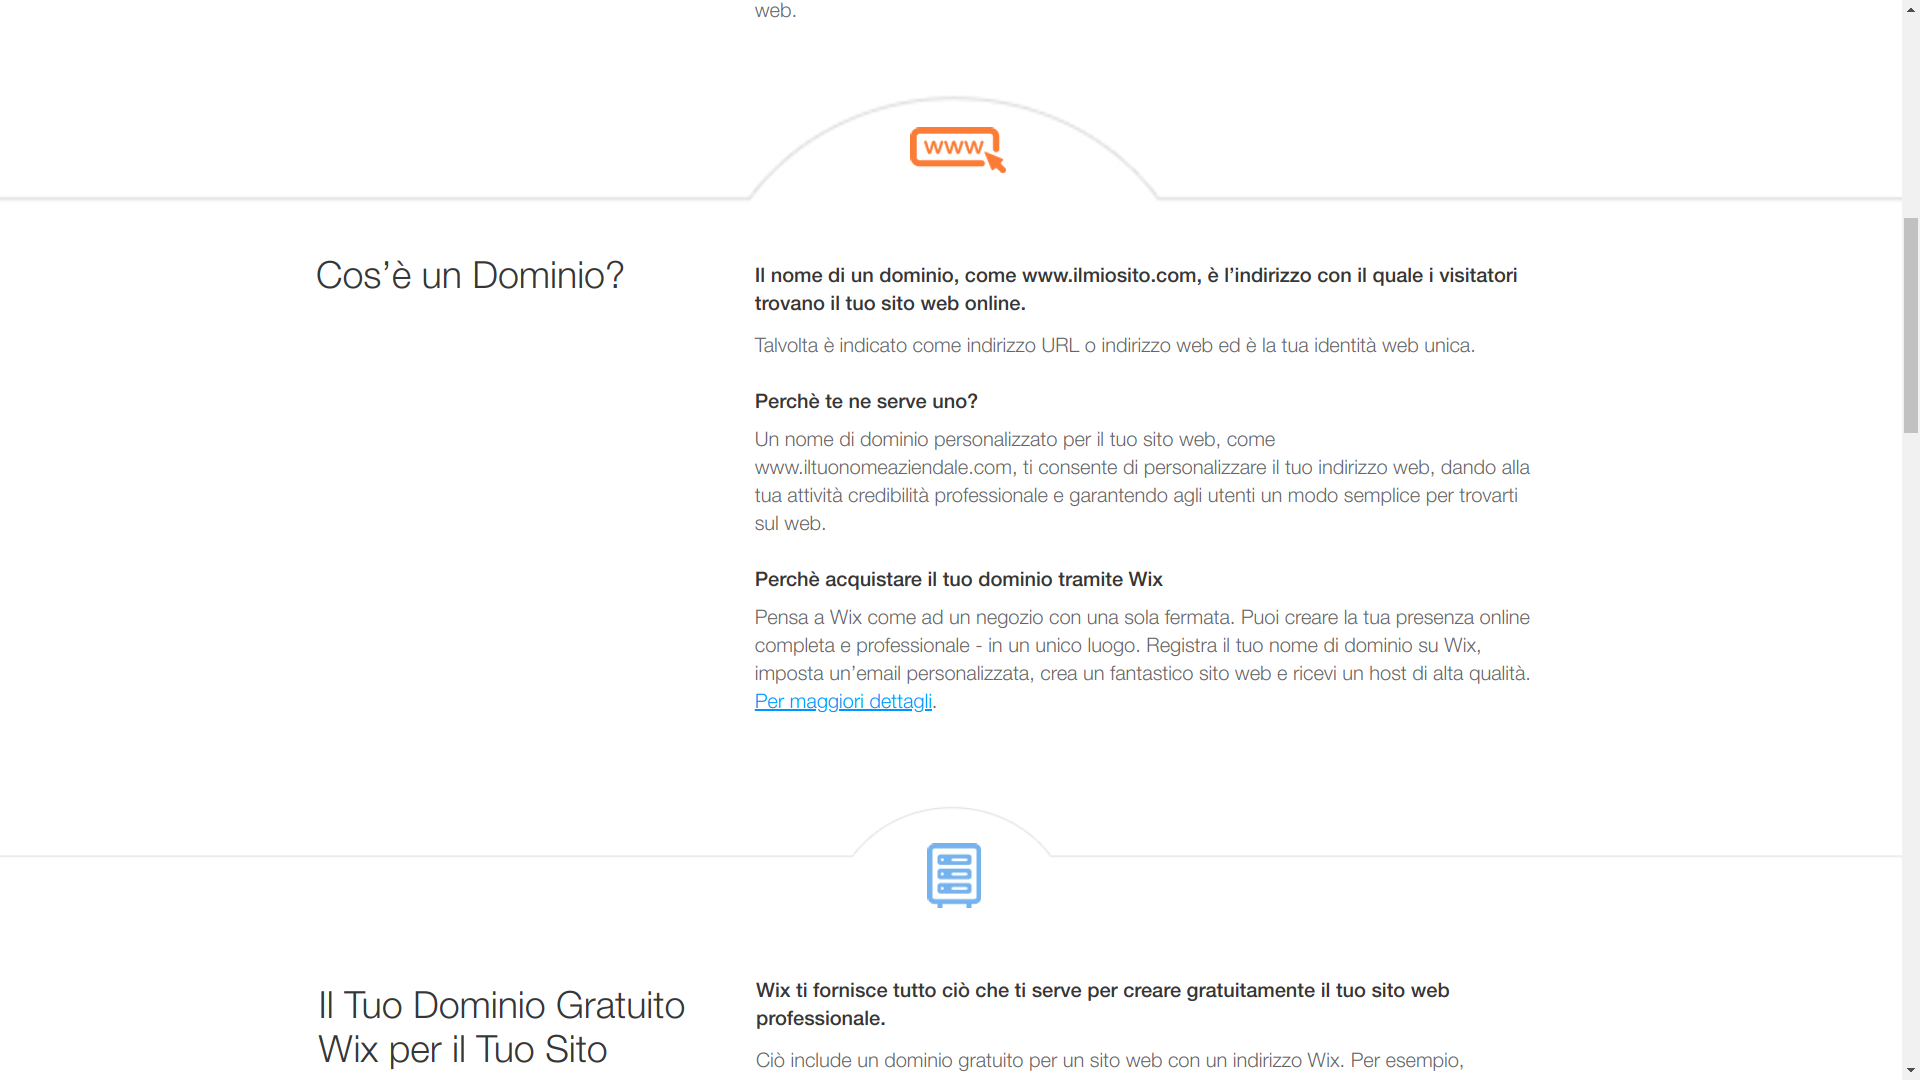
\includegraphics[width=1\textwidth]{img/domain-02.png}
  \caption{Dominio (pt. 2)}
  \label{fig:domain-02}
\end{figure}

Le schermate \ref{fig:domain-03} e \ref{fig:domain-04} proseguono con
un mix di informazioni sui contetti e, chiaramenti, consigli su
prodotti proprietari \wix{}.

\begin{figure}[H]
  \centering
  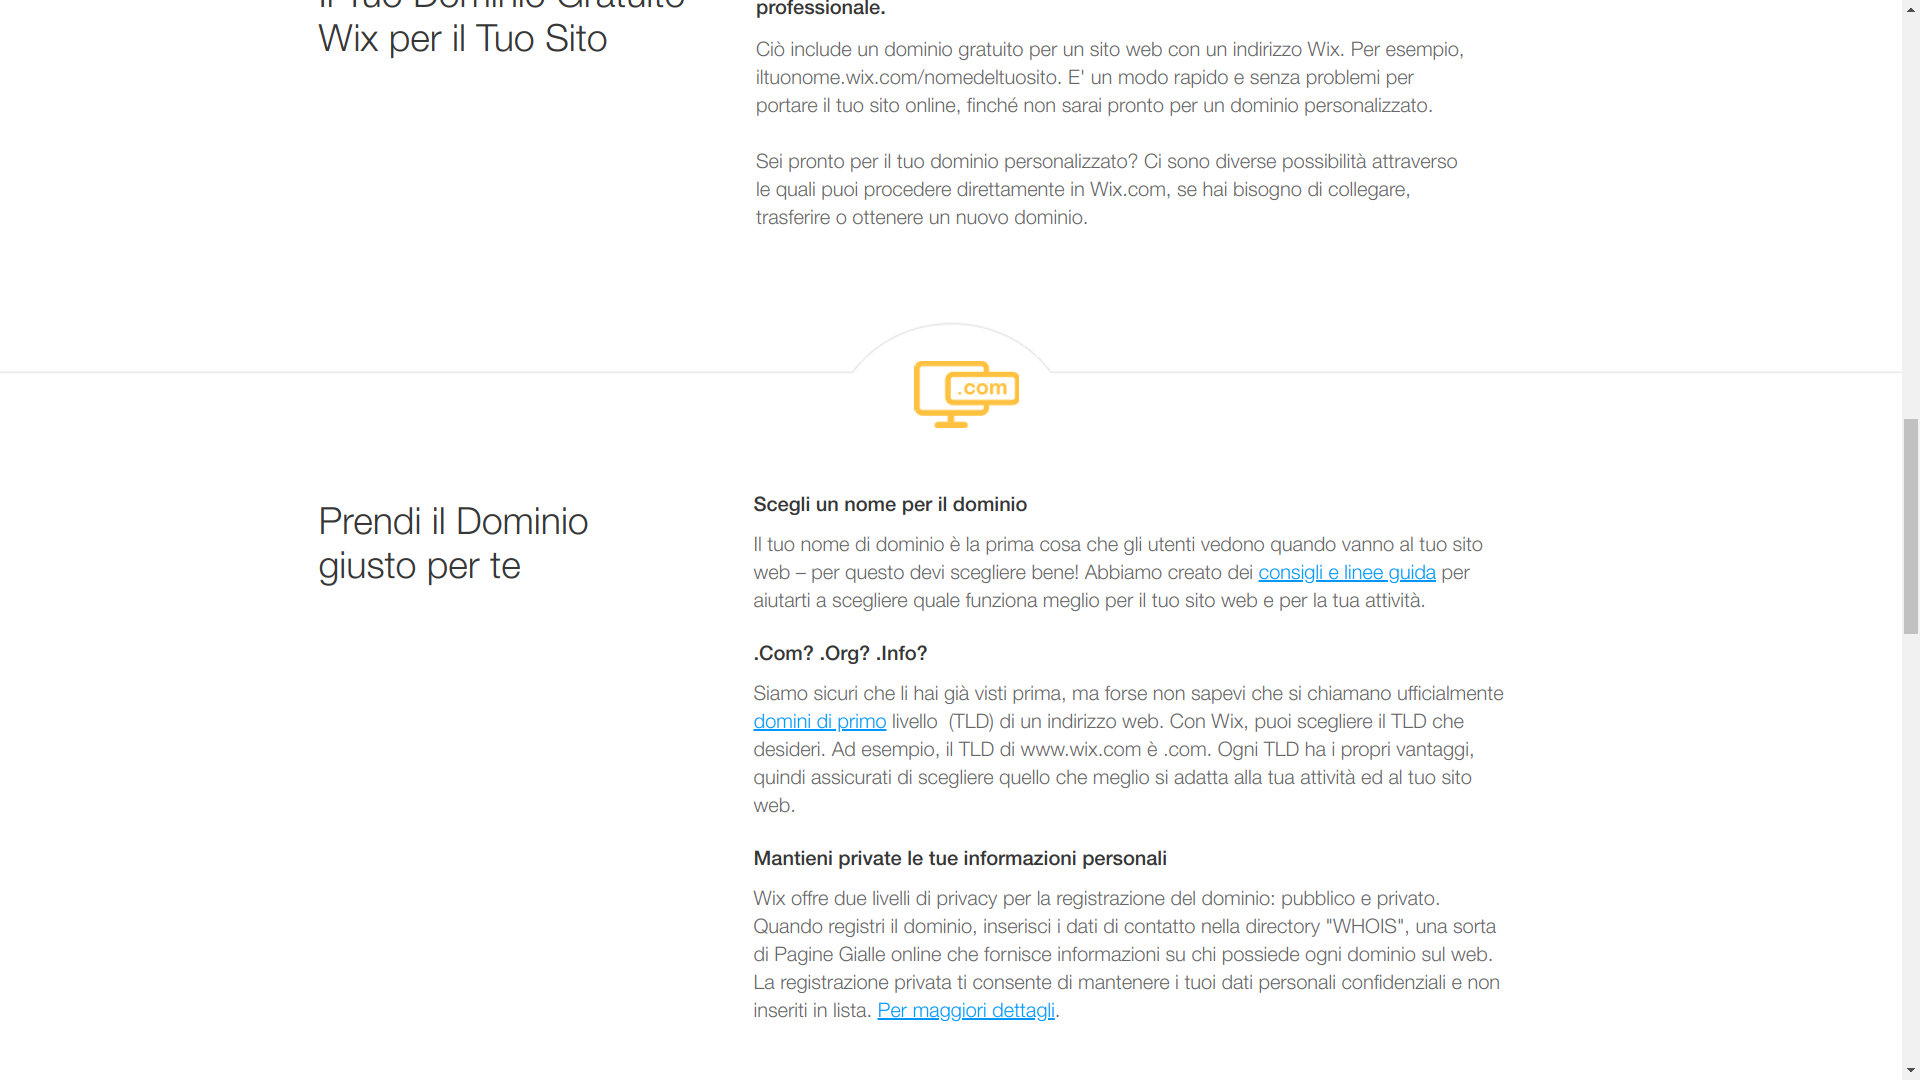
\includegraphics[width=1\textwidth]{img/domain-03.png}
  \caption{Dominio (pt. 3)}
  \label{fig:domain-03}
\end{figure}

\begin{figure}[H]
  \centering
  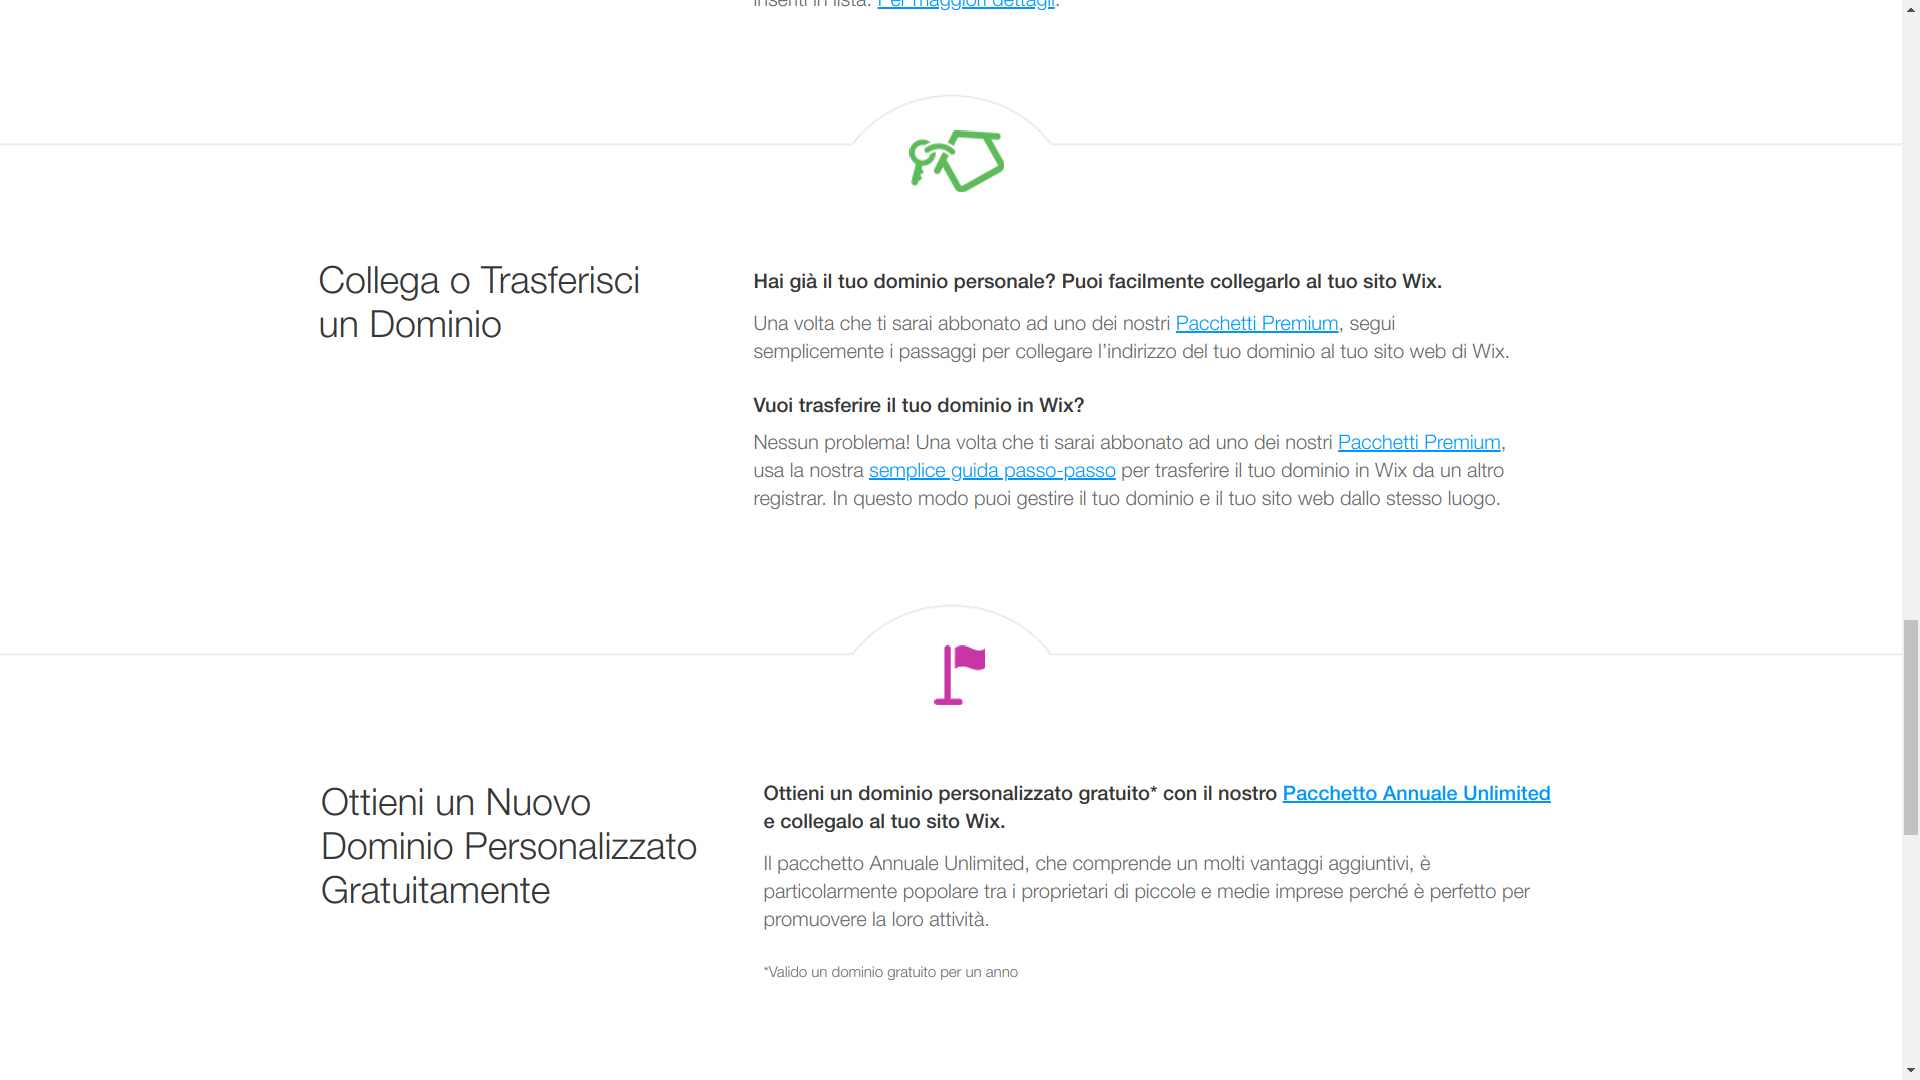
\includegraphics[width=1\textwidth]{img/domain-04.png}
  \caption{Dominio (pt. 4)}
  \label{fig:domain-04}
\end{figure}

La pagina termina poi con un footer del tutto simile a quello della
homepage, illustrato in figura \ref{fig:domain-05}.

\begin{figure}[H]
  \centering
  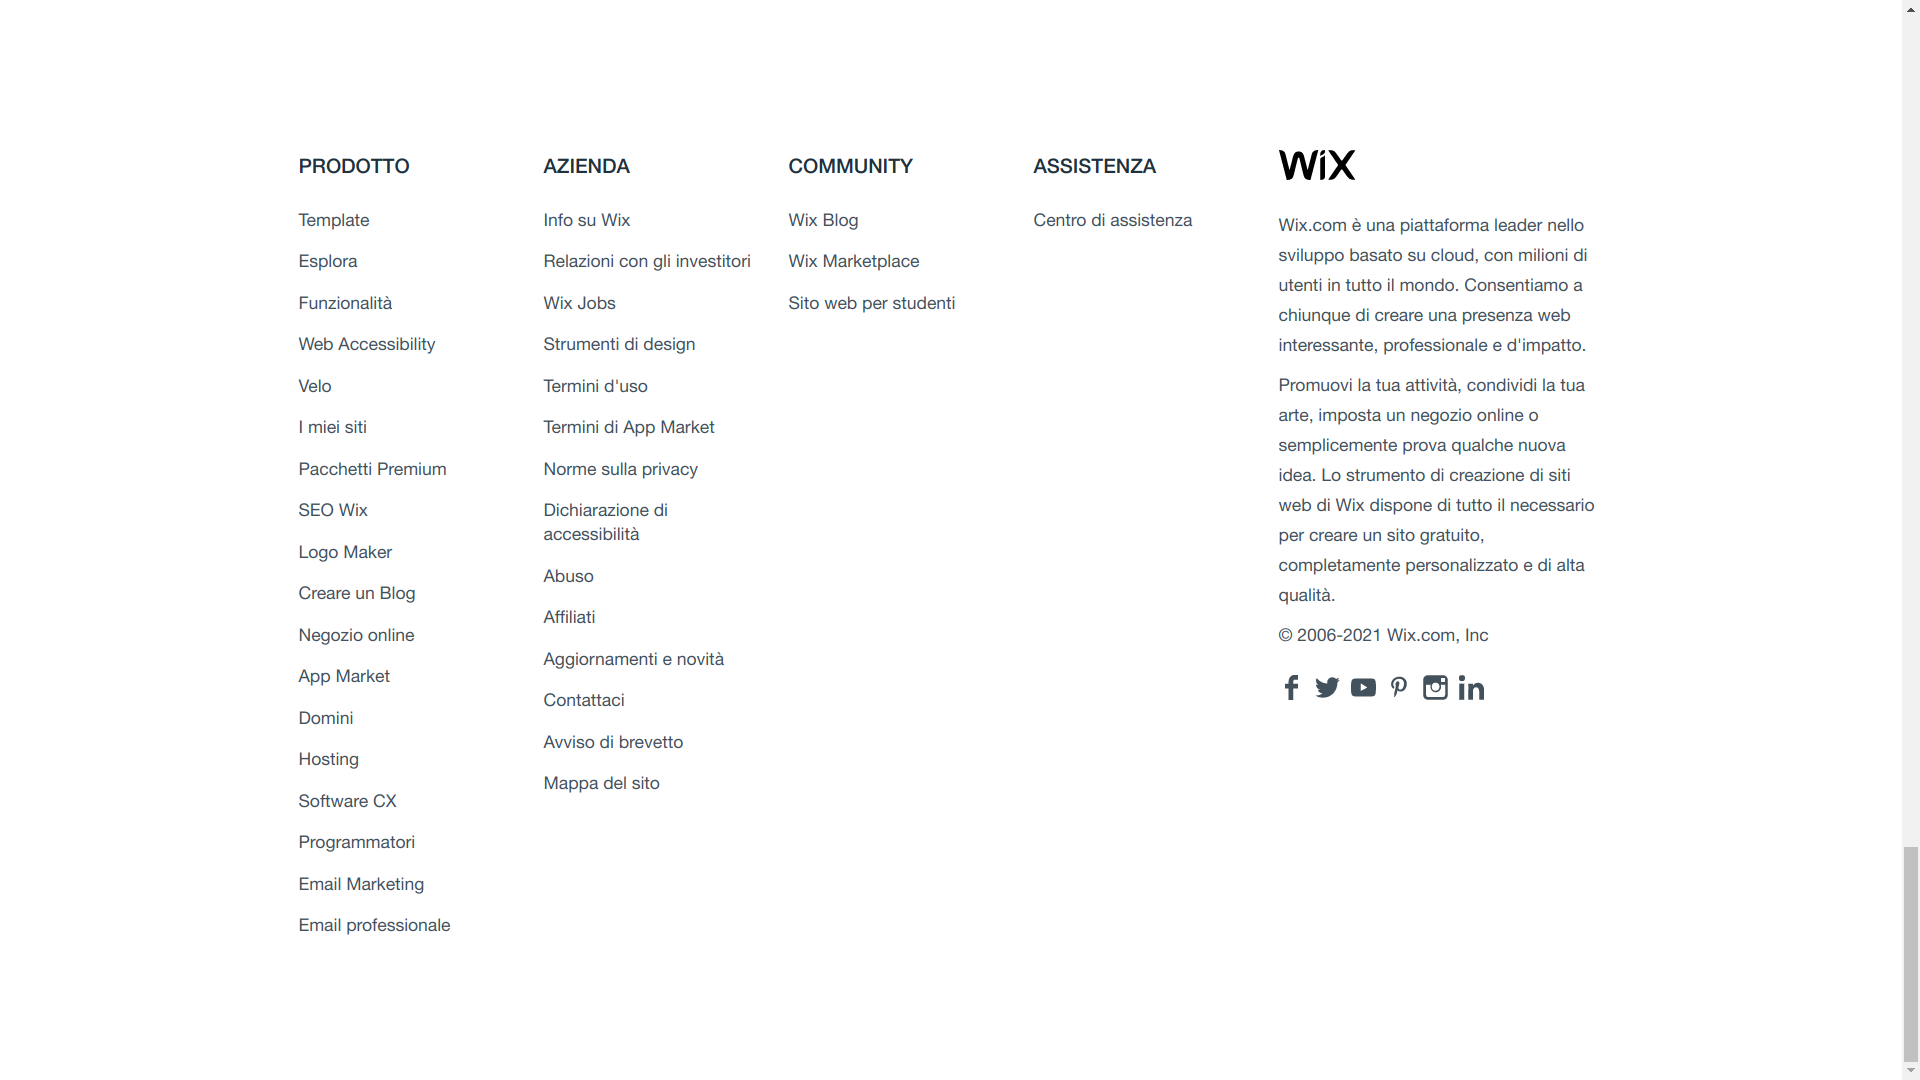
\includegraphics[width=1\textwidth]{img/domain-05.png}
  \caption{Dominio (pt. 5)}
  \label{fig:domain-05}
\end{figure}

\subsection{The Six Ws}
\label{subsec:internalpage-the-six-ws}

Analizziamo gli assi informativi della pagina interna.

\begin{itemize}
  \item \textbf{Where?} \textit{In quale sito web mi trovo?}
    L'immagine \ref{fig:domain-01} mostra la prima schemata della
    pagina interna ``Dominio''. Anche questa schemata, in stile
    homepage non è molto informativa, ma sicuramente dal logo in alto
    a sinistra l'utente capisce che è finito nel sito web di
    \wix{}. Non viene però approfondito che cos'è \wix{}.

  \item \textbf{Who?} \textit{Chi c'è dietro a questo sito?} Anche in
    questo caso l'informazione non è immediata e l'unico modo per
    rispondere esplicitamente alla domanda è arrivare al footer della
    pagina (figura \ref{fig:domain-05}).

  \item \textbf{Why?} \textit{Quali benefici offre il sito?} Le
    informazioni per rispondere alla domanda sono racchiuse nel titolo
    e nel sottotitolo (figura \ref{fig:domain-01}): la pagina offre un
    modo per promuovere l'attività tramite un dominio e gestirlo.

  \item \textbf{What?} \textit{Cosa viene offerto da questo sito?} La
    risposta viene parzialmente coperta dal titolo nella prima
    schermata (figura \ref{fig:domain-01}), ma in realtà la maggior
    parte delle informaizoni sono fornite successivamente in modo
    agevole dai titoli dei paragrafi: si fornisce un dominio gratuito
    per un sito web costruito con \wix{}, oppure il collegamento di un
    dominio esistente ad un sito \wix{} (figure \ref{fig:domain-02},
    \ref{fig:domain-03} e \ref{fig:domain-04}).

  \item \textbf{When?} \textit{Quali sono le ultime novità del sito?}
    La risposta nella pagina ``Dominio'' non è fornita e come per la
    homepage bisogna scorrere fino al footer ed identificare la voce
    \textit{Wix Blog} (figura \ref{fig:domain-05}).

  \item \textbf{How?} \textit{Come accedo alle funzionalità presentate
    dal sito?} Queste informazioni sono presenti nelle schermate
    riportate in figura \ref{fig:domain-02}, \ref{fig:domain-03} e
    \ref{fig:domain-04}, mescolate assieme alle informazioni dell'asse
    \textit{what}. In particolare ogni paragrafo, tranne ``Cos'è un
    Dominio?'' che è più di tipo informativo, mostra come accedere
    alle funzionalità presentate.
\end{itemize}

\section{Analisi complessiva}
\label{sec:full-analysis}

\subsection{Struttura}
\label{subsec:structure}

La struttura del sito web non è eccellente. Le informazioni sono
disperse nel layout bloated del sito web e ci sono diverse
informazioni difficili da reperire. La separazione del contenuto a
volte viene meno: una pagina per prodotto sarebbe stata sicuramente
più pulita, più chiara e non richiederebbe molti scroll per essere
letta.

\subsection{Layout}

Il layout del sito web è piuttosto bloated e privilegia spesso
l'aspetto visivo invece che favorire la lettura del contenuto. Ne è
un'esempio la homepage dove la prima schermata è completamente
dedicata ad un'immagine e alcune informazioni cruciali sono fornite
solo dopo diversi scroll.

\subsection{Navigazione}
\label{subsec:navigation}

La navigazione del sito \wix{} non è ottimale. Molti dei link di
\wix{} non sfruttano le convenzioni tradizionali dei link (colore blu
prima di essere visitati e viola dopo la visita), anzi. Spesso sono
bianchi se su sfondo scuro oppure nere su sfondo chiaro, proprio come
il testo. In questi casi però l'intuizione dell'utente è aiutata da
sottolineatura e dal simbolo di una ``freccina''. Altri link,
principalmente call-to-action, sono trasformati in pulsanti, rendendo
invece chiara l'intenzione del componente.

\begin{figure}[H]
  \centering
  
\includegraphics[]{img/link-btn.png}
  \caption{Link a forma di pulsante}
  \label{fig:link-btn}
\end{figure}

\begin{figure}[H]
  \centering
  
\includegraphics[]{img/link-white-on-blue-underline.png}
  \caption{Link bianco su blu con enfasi}
  \label{fig:link-white-on-blue-underline}
\end{figure}

\begin{figure}[H]
  \centering
  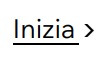
\includegraphics[]{img/link-black-on-white-underline.png}
  \caption{Link nero su bianco con enfasi}
  \label{fig:black-on-white-underline}
\end{figure}

\begin{figure}[H]
  \centering
  
\includegraphics[]{img/link-text.png}
  \caption{Link immerso nel testo}
  \label{fig:link-text}
\end{figure}

Il menu di navigazione in alto al sito è molto standard ma presenta un
problema fondamentale: ogni voce del menu apre una nuova
scheda. Questo in termini di usabilità è molto impattante in quanto
viene meno la funzione back del browser: le nuove schede del browser
resettano la storia di navigazione. Ciò significa che l'utente non può
ricorrere all'algoritmica low-cost per cercare tramite backtracking
informazioni, oltre al fatto che molte tab del browser confondono
l'utente medio.

\begin{figure}[H]
  \centering
  
\includegraphics[width=1\textwidth]{img/navbar.png}
  \caption{Menu di navigazione}
  \label{fig:navbar}
\end{figure}

Il sito web non presenta nessun aiuto alla navigazione con la tecnica
breadcrumb, anche non ci sono forti gerarchie di pagine per le quali
la breadcrumb sarebbe necessaria.

Altro grande assente sul sito web \wix{} è la funzionalità di
ricerca. Seppur \wix{} abbia diversi prodotti e abbia diverse
informazioni sul proprio sito web, compreso il supporto con guide e
tutorial per lo sviluppo del proprio sito web, non viene offerta una
funzionalità di ricerca sul primo livello del sito web. Solo la pagina
``Assistenza'' è fornita di questa funzionalità, ma chiaramente la
ricerca in questo caso trova solo gli articoli con la documentazione
su \wix{}, non cerca informazioni sul sito.

\begin{figure}[H]
  \centering
  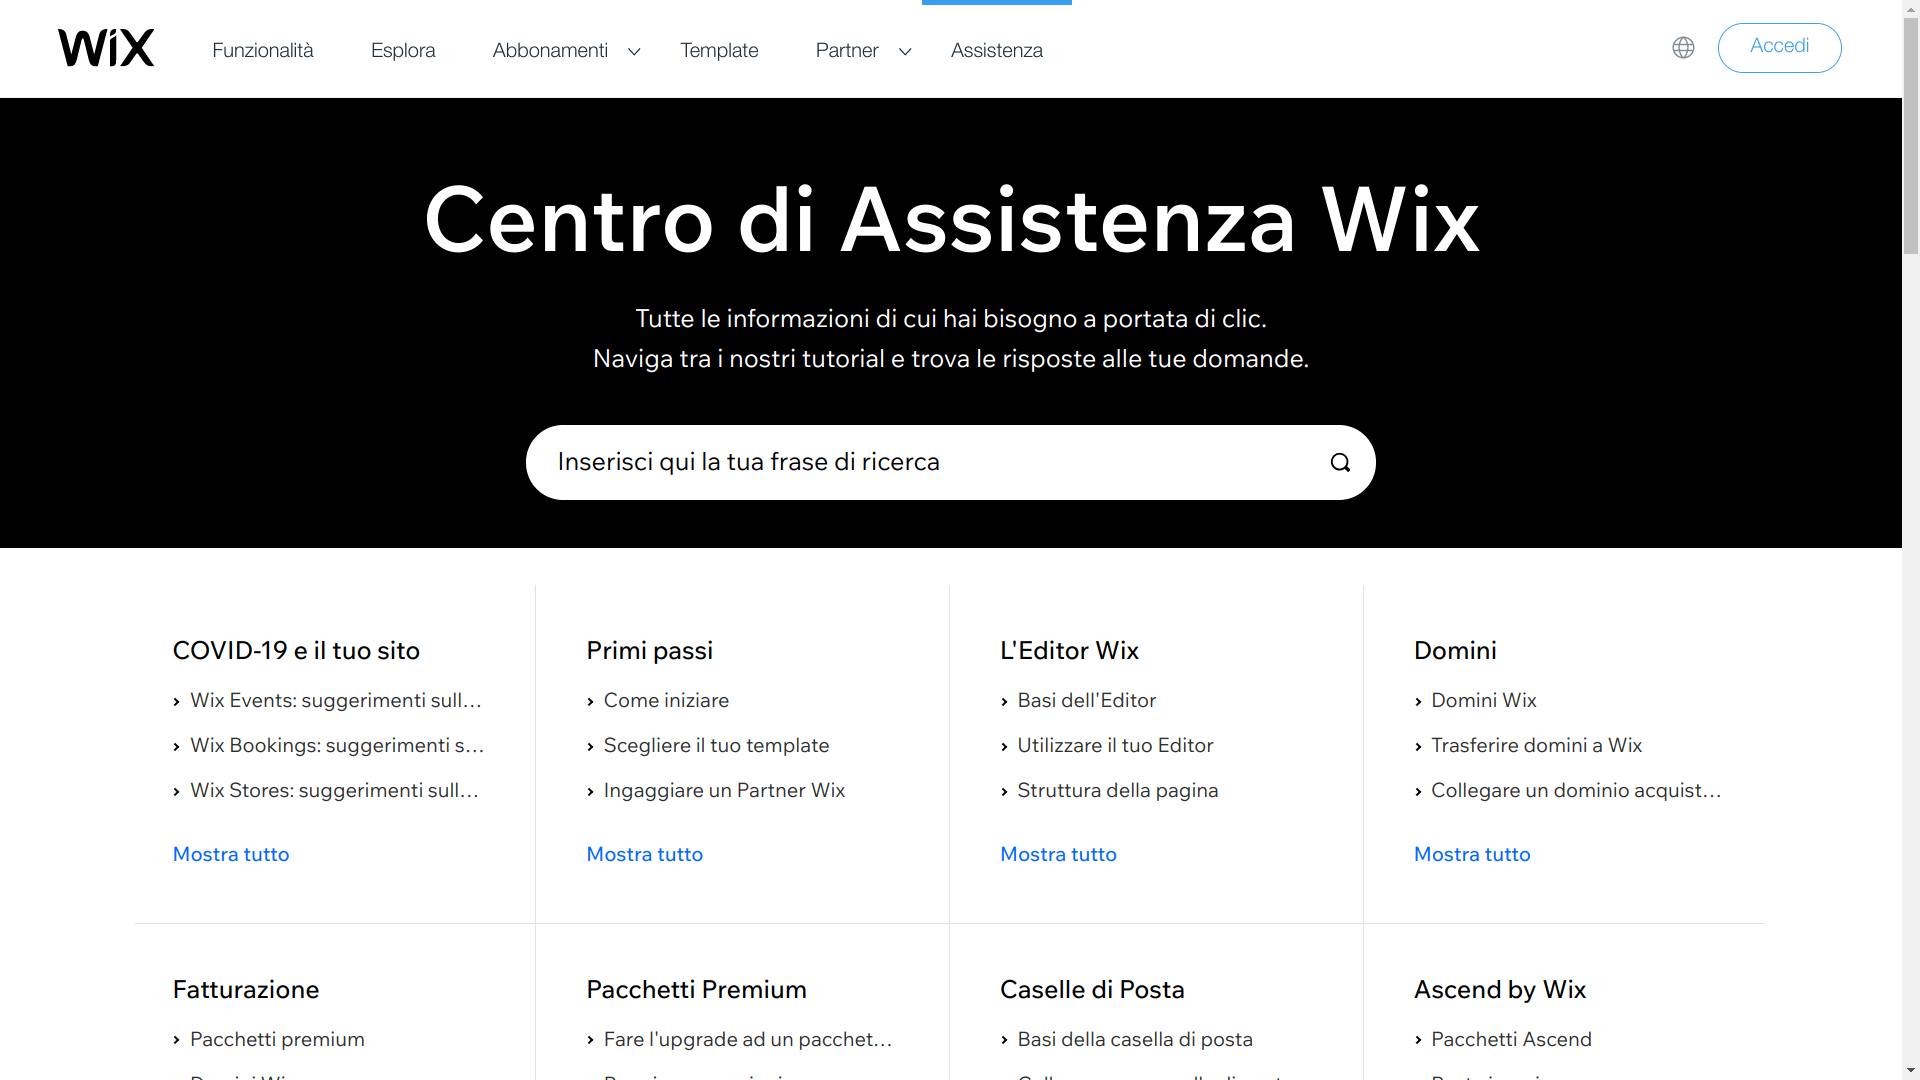
\includegraphics[width=1\textwidth]{img/search-bar.png}
  \caption{Barra di ricerca della pagina assistenza}
  \label{fig:search-bar}
\end{figure}

Inoltre, la barra di ricerca, come mostra la figura
\ref{fig:search-bar} non è standard: il pulsante per cercare non
esiste e l'icona con la lente di ingrandimento è una metafora tradita:
non può essere cliccata. Non esiste nemmeno il supporto alla pressione
del tasto \textit{enter}. Di fatto, per cercare bisogna digitare una
query e solo a questo punto premere sulla lente di ingrandimento (ora
colorata di blu) oppure direttamente su uno dei risultato rapidi.

\begin{figure}[H]
  \centering
  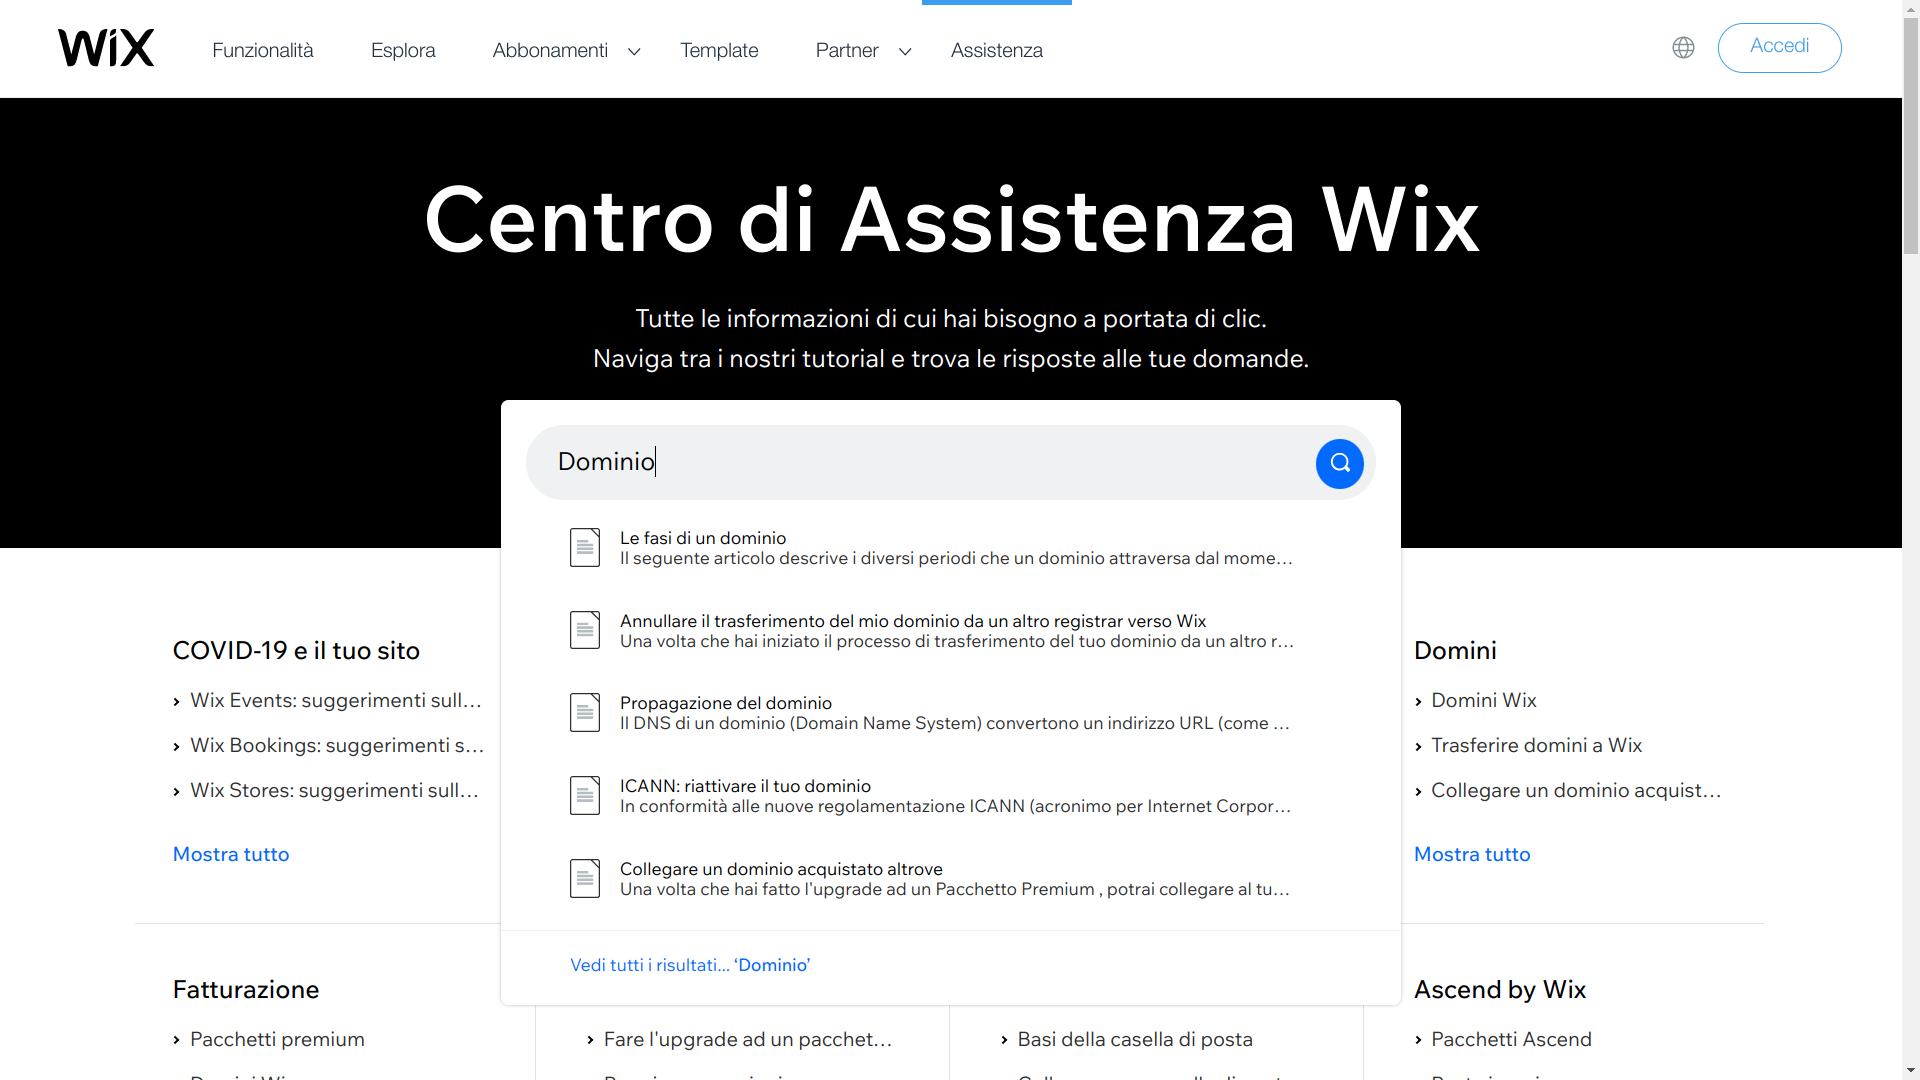
\includegraphics[width=1\textwidth]{img/search-bar-results.png}
  \caption{Utilizzo della barra di ricerca della pagina assistenza}
  \label{fig:search-bar-results}
\end{figure}

\subsection{Pubblicità}
\label{subsec:ads}

Il sito web non presenta pubblicità essendo un sito con lo scopo di
presentare il proprio prodotto e aggiungere pubblicità anche se non
troppo fastidiosa potrebbe essere controproducente.

\subsection{Immagini}
\label{subsec:images}

Le immagini di \wix{} sono molto curate in termini di impatti visivo
ma veramente poco funzionali in termini dell'usabilità del sito
web. Tendono spesso a confodere il lettore e occupano molto spazio
prezioso.

\subsection{Registrazione}
\label{subsec:signup}

Praticamente ogni link ``Inizia ora'' porta alla pagina di
registrazione. Questo link è presente anche nella prima schermata
della homepage (figura \ref{fig:homepage-01}): siamo di fronte al
fenomeno della registrazione prematura.

\begin{figure}[H]
  \centering
  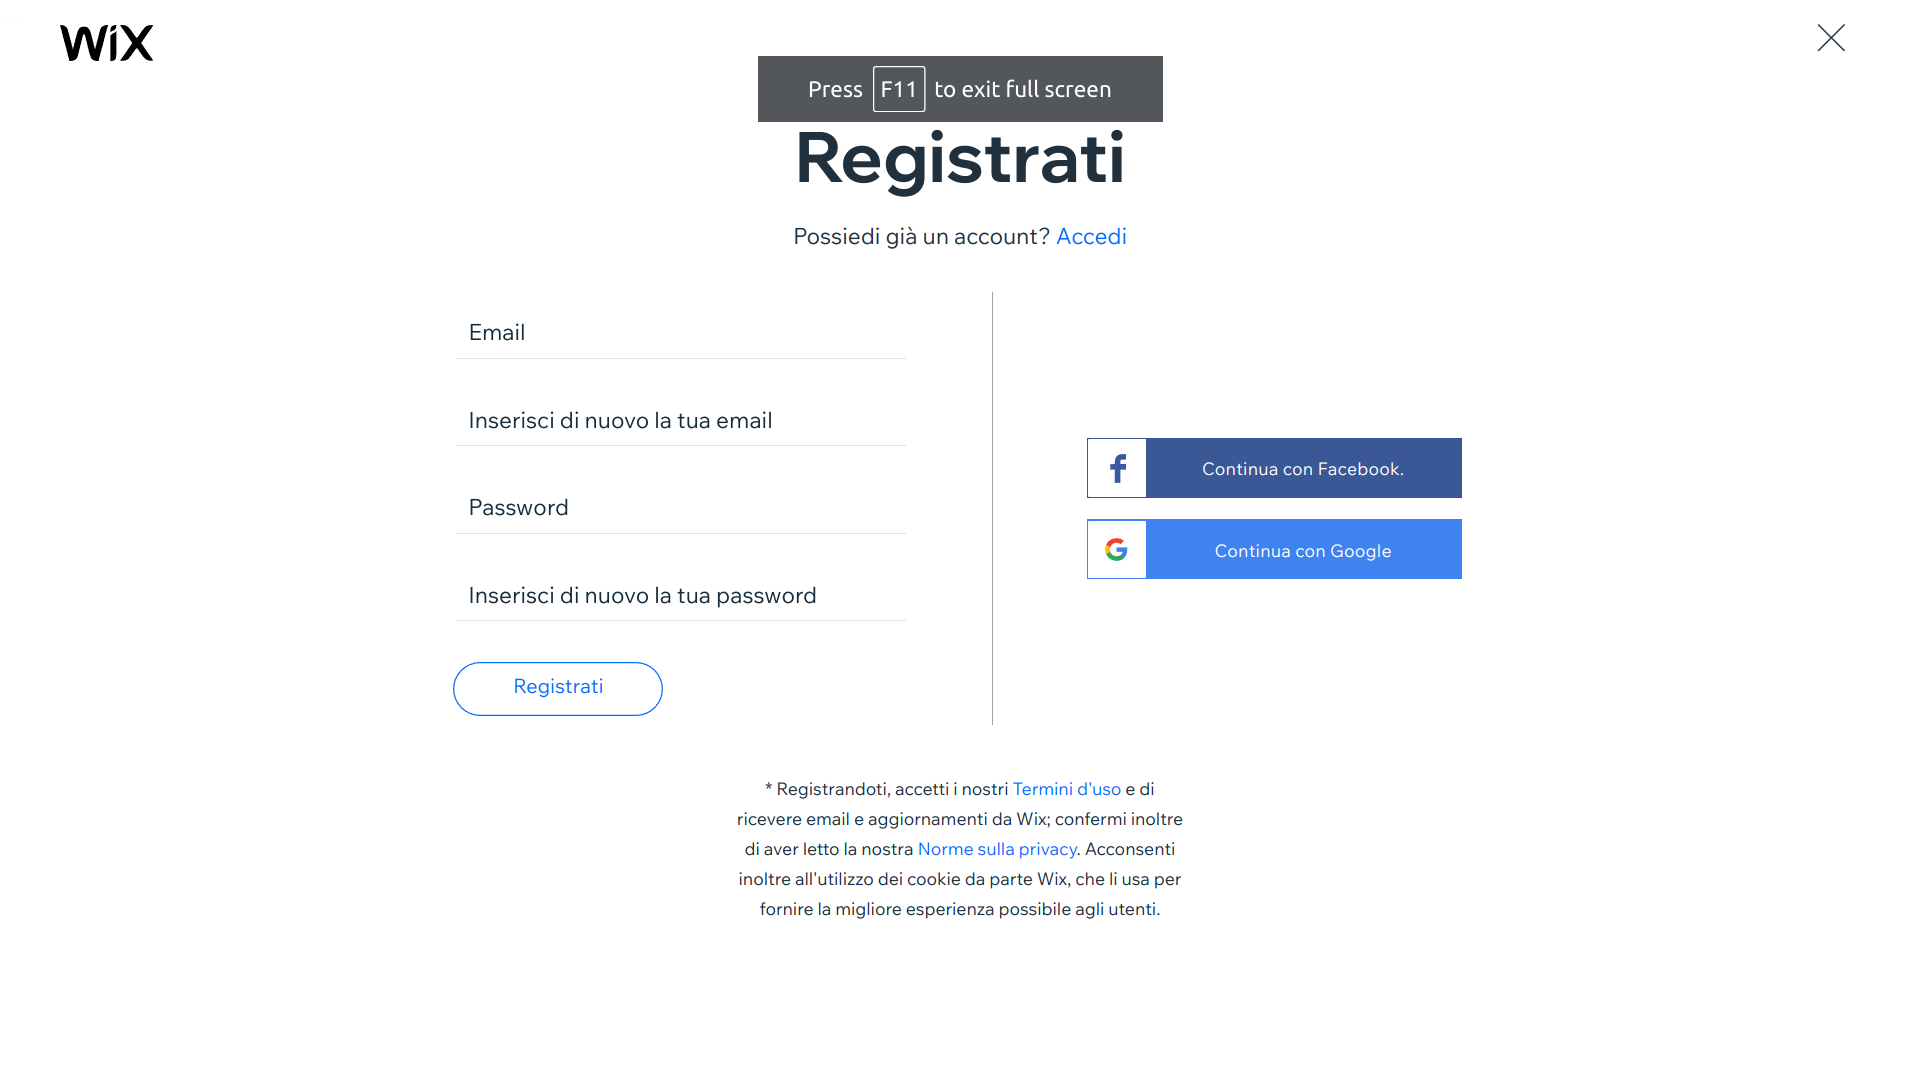
\includegraphics[width=1\textwidth]{img/registration.png}
  \caption{Form di registrazione}
  \label{fig:registration}
\end{figure}

\section{Altre pagine}
\label{sec:other-pages}

Degna di nota è la pagina delle funzionalità: essa presenta i vari
prodotti associati a \wix{}. Per visitare questa pagina completamente
bisogna però effettuare ben ventiquattro scroll (sic!). In alto alla
pagina è presente un mini-menu per la navigazione della stessa, ma
ventiquattro scroll sono comunque troppi.

\section{Considerazioni finali}
\label{sec:final-remarks}

Trovo \wix{} un sito web molto carente dal punto di vista
dell'usabilità utente. Mi sarei aspettato, da un'azienda che permette
di realizzare siti web ai suoi utenti, che fossero a conoscenza di
tutte le regole di usabilità e ingaggio. Alcune di queste invece sono
ignorate e anche se il layout e l'apparenza del sito sono molto
gradevoli alla vista, la frustrazione cresce ad ogni secondo di
utilizzo del sito web. 

A parere mio andrebbero riviste diverse sezioni e riorganizzata la
struttura del sito web, ricorrendo ad un layout meno bloated che
privilegi l'informazione piuttosto che l'immagine perfetta. 

\section{Giudizio finale}
\label{sec:final-vote}

Vengono riportati nella tabella i vari ambiti considerati nell'analisi
e la loro valutazione. Segue il giudizio finale (che non è la semplice
media delle varie valutazioni nella tabella) con un riassunto delle
motivazioni.

\begin{table}
  \centering
  \begin{tabular}{||l|r||}
    \hline
    \textbf{Ambito} & \textbf{Valutazione} \\
    \hline\hline
     Homepage & 2 \\ 
     Pagina interna & 7 \\
     Layout & 4 \\
     Struttura & 6 \\
     Immagini & 4 \\
     Navigazione & 5 \\
     Contenuti & 6 \\
     \hline\hline
     Giudizio finale & 4 \\
     \hline
  \end{tabular}
  \caption{Valutazione del sito web}
  \label{table:rating}
\end{table}

Molto penalizzante è sicuramente il giudizio della homepage, ma,
secondo me, la pagina più importante del sito è quella strutturata
peggio e dove si trovano informazioni rilevanti solo dopo molti scroll
o non si trovano affatto. Come ho già detto diverse volte immagini e
layout bloated non sono di aiuto in alcun modo al contenuto, che
rimane comunque povero. \'E stato fatto un buon lavoro invece nella
pagina interna dove le informazioni sono ben strutturate e facilmente
reperibili. La navigazione non è sufficiente per le troppe
imprecisioni, soprattutto per quanto riguarda il menu di
navigazione. In conclusione, sommando tutte le imprecisioni il sito
web risulta poco usabile.

\section{Aggiornamento marzo 2021}

Durante l'analisi di \wix{}, il sito ha subito un'aggiornamento della
veste grafica riguardante principalmente la homepage. La figura
\ref{fig:homepage-updated} mostra la modifica. In questa versione il
titolo della pagina (rimasto lo stesso rispetto alla versione
precedente) è più enfatizzato e attira molto l'attenzione da parte
dell'utente. Inoltre esso è aiutato da un sottotitolo che in un paio
di righe riassume gli assi \textit{why} e \textit{what}.

\begin{figure}[H]
  \centering
  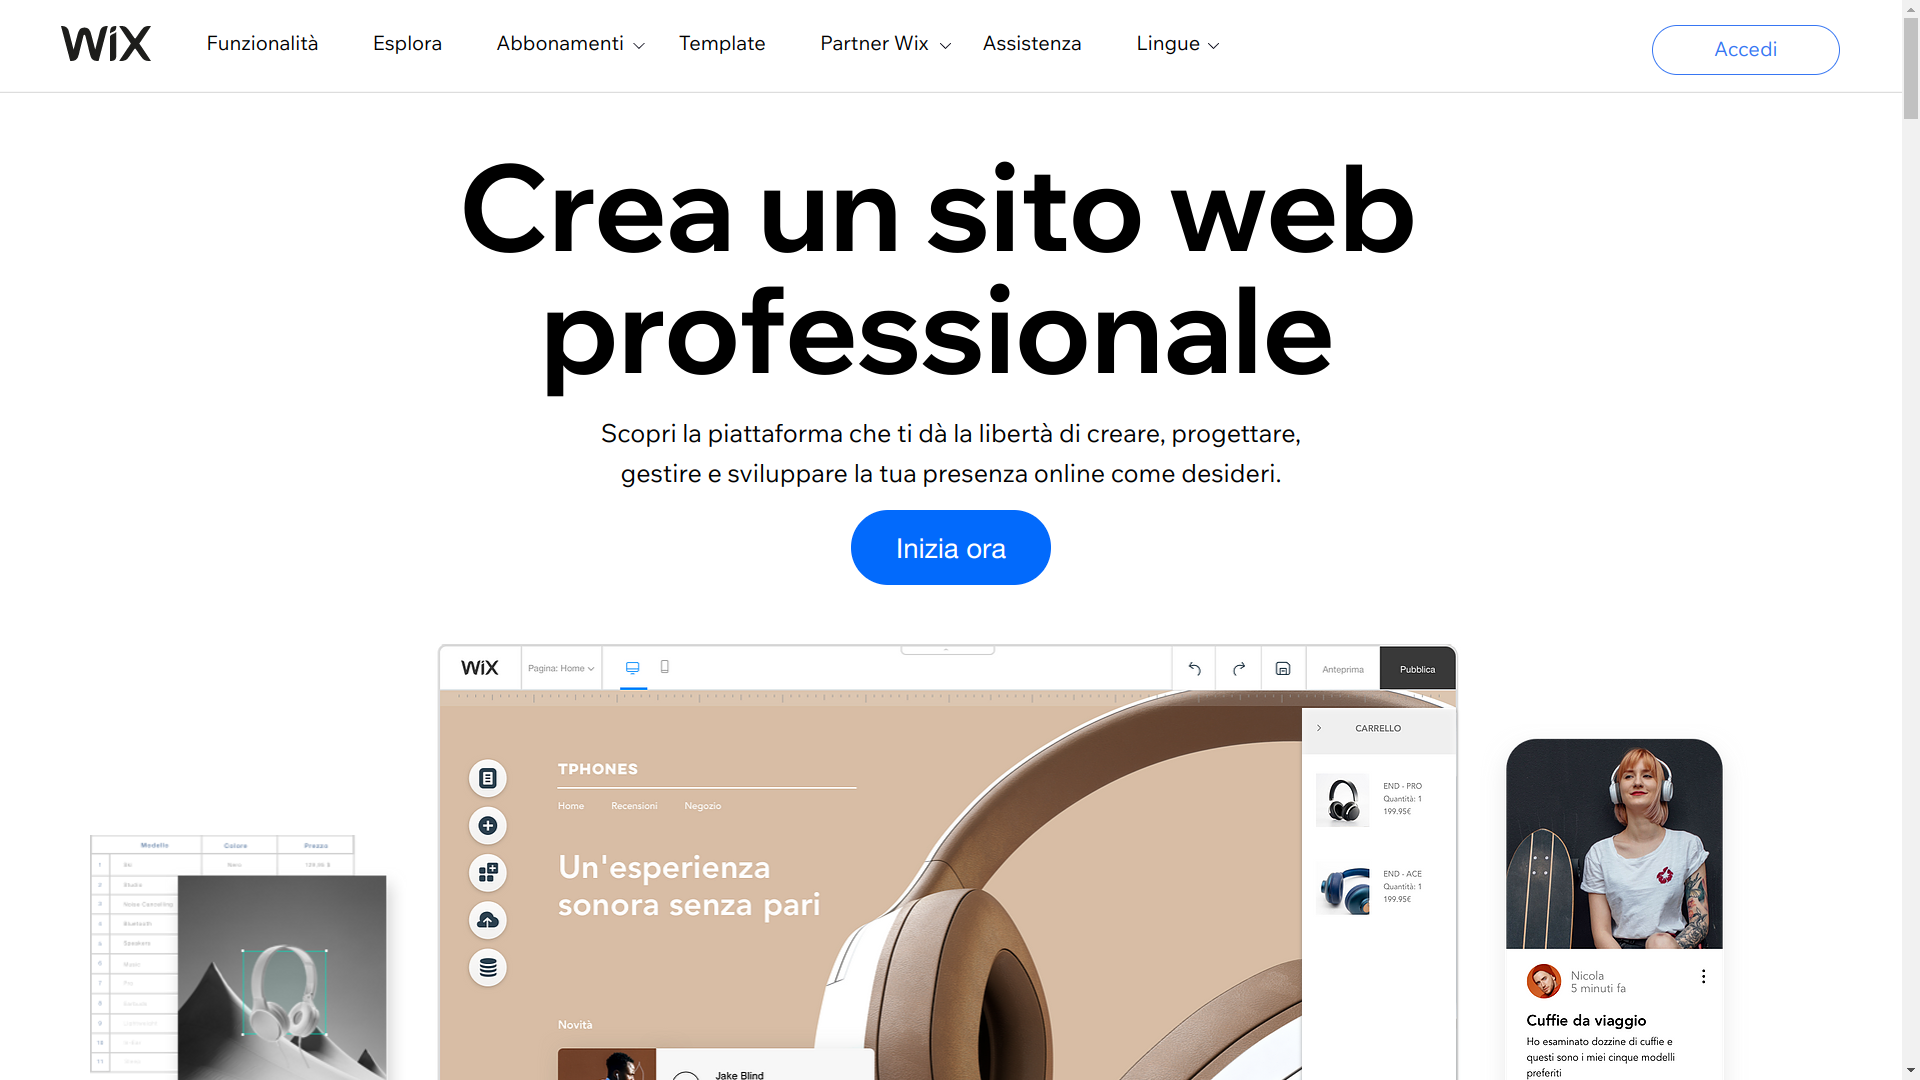
\includegraphics[width=1\textwidth]{img/homepage-updated.png}
  \caption{Homepage aggiornata}
  \label{fig:homepage-updated}
\end{figure}

\section{Lista delle figure}

Nota: i valori della colonna \textit{Pagina} si riferiscono agli URL
riportati di seguito.

\begin{itemize}
  \item assistenza = \url{https://support.wix.com/it/}
  \item dominio = \url{https://it.wix.com/domain/names}
  \item homepage = \url{https://it.wix.com/}
  \item registrazione = \url{https://wix.com/signin}
\end{itemize}

\begin{table}[]
  \centering
  \begin{tabular}{||p{4cm}|c|c||}
    \hline
    \textbf{Figura} & \textbf{File} & \textbf{Pagina} \\
    \hline\hline
     Dominio (pt. 1) & domain-01.png & dominio \\
     Dominio (pt. 2) & domain-02.png & dominio \\
     Dominio (pt. 3) & domain-03.png & dominio \\
     Dominio (pt. 4) & domain-04.png & dominio \\
     Dominio (pt. 5) & domain-05.png & dominio \\
     Homepage (pt. 1) & homepage-01.png & homepage \\
     Homepage (pt. 2) & homepage-02.png & homepage \\
     Homepage (pt. 3) & homepage-03.png & homepage \\
     Homepage (pt. 4) & homepage-04.png & homepage \\
     Homepage (pt. 5) & homepage-05.png & homepage \\
     Homepage (pt. 6) & homepage-06.png & homepage \\
     Homepage (pt. 7) & homepage-07.png & homepage \\
     Homepage (pt. 8) & homepage-08.png & homepage \\
     Homepage (pt. 9) & homepage-09.png & homepage \\
     Homepage (pt. 10) & homepage-10.png & homepage \\
     Homepage (pt. 11) & homepage-11.png & homepage \\
     Homepage aggiornata & homepage-updated.png & homepage \\
     Link nero su bianco con enfasi & link-black-on-white-underline.png & homepage \\
     Link a forma di pulsante & link-btn.png & homepage \\
     Link immerso nel testo & link-text.png & dominio \\
     Link bianco su blu con enfasi & link-white-on-blue-underline.png & homepage \\
     Menu di navigazione & navbar.png & homepage \\
     Form di registrazione & registration.png & registrazione \\
     Barra di ricerca della pagina assistenza & search-bar.png & assistenza \\
     Utilizzo della barra di ricerca della pagina assistenza & search-bar-results.png & assistenza \\
     Logo di Wix & wix-logo.png & homepage \\
     \hline
  \end{tabular}
  \caption{Lista delle figure}
  \label{table:list-of-figures}
\end{table}

\end{document}
